\documentclass[
  shownotes,
  xcolor={svgnames},
  hyperref={colorlinks,citecolor=DarkBlue,linkcolor=DarkRed,urlcolor=DarkBlue}
  , aspectratio=169]{beamer}
\usepackage{animate}
\usepackage{amsmath}
\usepackage{amsfonts}
\usepackage{amssymb}
\usepackage{pifont}
\usepackage{mathpazo}
%\usepackage{xcolor}
\usepackage{multimedia}
\usepackage{fancybox}
\usepackage[para]{threeparttable}
\usepackage{multirow}
\setcounter{MaxMatrixCols}{30}
\usepackage{subcaption}
\usepackage{graphicx}
\usepackage{lscape}
\usepackage[compatibility=false,font=small]{caption}
\usepackage{booktabs}
\usepackage{ragged2e}
\usepackage{chronosys}
\usepackage{appendixnumberbeamer}
\usepackage{animate}
\setbeamertemplate{caption}[numbered]
\usepackage{color}
%\usepackage{times}
\usepackage{tikz}
\usepackage{comment} %to comment
%% BibTeX settings
\usepackage{natbib}
\bibliographystyle{apalike}
\bibpunct{(}{)}{,}{a}{,}{,}
\setbeamertemplate{bibliography item}{[\theenumiv]}

% Defines columns for bespoke tables
\usepackage{array}
\newcolumntype{L}[1]{>{\raggedright\let\newline\\\arraybackslash\hspace{0pt}}m{#1}}
\newcolumntype{C}[1]{>{\centering\let\newline\\\arraybackslash\hspace{0pt}}m{#1}}
\newcolumntype{R}[1]{>{\raggedleft\let\newline\\\arraybackslash\hspace{0pt}}m{#1}}


\usepackage{xfrac}


\usepackage{multicol}
\setlength{\columnsep}{0.5cm}

% Theme and colors
\usetheme{Boadilla}

% I use steel blue and a custom color palette. This defines it.
\definecolor{andesred}{HTML}{af2433}

% Other options
\providecommand{\U}[1]{\protect\rule{.1in}{.1in}}
\usefonttheme{serif}
\setbeamertemplate{itemize items}[default]
\setbeamertemplate{enumerate items}[square]
\setbeamertemplate{section in toc}[circle]

\makeatletter

\definecolor{mybackground}{HTML}{82CAFA}
\definecolor{myforeground}{HTML}{0000A0}

\setbeamercolor{normal text}{fg=black,bg=white}
\setbeamercolor{alerted text}{fg=red}
\setbeamercolor{example text}{fg=black}

\setbeamercolor{background canvas}{fg=myforeground, bg=white}
\setbeamercolor{background}{fg=myforeground, bg=mybackground}

\setbeamercolor{palette primary}{fg=black, bg=gray!30!white}
\setbeamercolor{palette secondary}{fg=black, bg=gray!20!white}
\setbeamercolor{palette tertiary}{fg=white, bg=andesred}

\setbeamercolor{frametitle}{fg=andesred}
\setbeamercolor{title}{fg=andesred}
\setbeamercolor{block title}{fg=andesred}
\setbeamercolor{itemize item}{fg=andesred}
\setbeamercolor{itemize subitem}{fg=andesred}
\setbeamercolor{itemize subsubitem}{fg=andesred}
\setbeamercolor{enumerate item}{fg=andesred}
\setbeamercolor{item projected}{bg=gray!30!white,fg=andesred}
\setbeamercolor{enumerate subitem}{fg=andesred}
\setbeamercolor{section number projected}{bg=gray!30!white,fg=andesred}
\setbeamercolor{section in toc}{fg=andesred}
\setbeamercolor{caption name}{fg=andesred}
\setbeamercolor{button}{bg=gray!30!white,fg=andesred}


\usepackage{fancyvrb}
\newcommand{\VerbBar}{|}
\newcommand{\VERB}{\Verb[commandchars=\\\{\}]}
\DefineVerbatimEnvironment{Highlighting}{Verbatim}{commandchars=\\\{\}}
% Add ',fontsize=\small' for more characters per line
\usepackage{framed}
\definecolor{shadecolor}{RGB}{248,248,248}
\newenvironment{Shaded}{\begin{snugshade}}{\end{snugshade}}
\newcommand{\AlertTok}[1]{\textcolor[rgb]{0.94,0.16,0.16}{#1}}
\newcommand{\AnnotationTok}[1]{\textcolor[rgb]{0.56,0.35,0.01}{\textbf{\textit{#1}}}}
\newcommand{\AttributeTok}[1]{\textcolor[rgb]{0.77,0.63,0.00}{#1}}
\newcommand{\BaseNTok}[1]{\textcolor[rgb]{0.00,0.00,0.81}{#1}}
\newcommand{\BuiltInTok}[1]{#1}
\newcommand{\CharTok}[1]{\textcolor[rgb]{0.31,0.60,0.02}{#1}}
\newcommand{\CommentTok}[1]{\textcolor[rgb]{0.56,0.35,0.01}{\textit{#1}}}
\newcommand{\CommentVarTok}[1]{\textcolor[rgb]{0.56,0.35,0.01}{\textbf{\textit{#1}}}}
\newcommand{\ConstantTok}[1]{\textcolor[rgb]{0.00,0.00,0.00}{#1}}
\newcommand{\ControlFlowTok}[1]{\textcolor[rgb]{0.13,0.29,0.53}{\textbf{#1}}}
\newcommand{\DataTypeTok}[1]{\textcolor[rgb]{0.13,0.29,0.53}{#1}}
\newcommand{\DecValTok}[1]{\textcolor[rgb]{0.00,0.00,0.81}{#1}}
\newcommand{\DocumentationTok}[1]{\textcolor[rgb]{0.56,0.35,0.01}{\textbf{\textit{#1}}}}
\newcommand{\ErrorTok}[1]{\textcolor[rgb]{0.64,0.00,0.00}{\textbf{#1}}}
\newcommand{\ExtensionTok}[1]{#1}
\newcommand{\FloatTok}[1]{\textcolor[rgb]{0.00,0.00,0.81}{#1}}
\newcommand{\FunctionTok}[1]{\textcolor[rgb]{0.00,0.00,0.00}{#1}}
\newcommand{\ImportTok}[1]{#1}
\newcommand{\InformationTok}[1]{\textcolor[rgb]{0.56,0.35,0.01}{\textbf{\textit{#1}}}}
\newcommand{\KeywordTok}[1]{\textcolor[rgb]{0.13,0.29,0.53}{\textbf{#1}}}
\newcommand{\NormalTok}[1]{#1}
\newcommand{\OperatorTok}[1]{\textcolor[rgb]{0.81,0.36,0.00}{\textbf{#1}}}
\newcommand{\OtherTok}[1]{\textcolor[rgb]{0.56,0.35,0.01}{#1}}
\newcommand{\PreprocessorTok}[1]{\textcolor[rgb]{0.56,0.35,0.01}{\textit{#1}}}
\newcommand{\RegionMarkerTok}[1]{#1}
\newcommand{\SpecialCharTok}[1]{\textcolor[rgb]{0.00,0.00,0.00}{#1}}
\newcommand{\SpecialStringTok}[1]{\textcolor[rgb]{0.31,0.60,0.02}{#1}}
\newcommand{\StringTok}[1]{\textcolor[rgb]{0.31,0.60,0.02}{#1}}
\newcommand{\VariableTok}[1]{\textcolor[rgb]{0.00,0.00,0.00}{#1}}
\newcommand{\VerbatimStringTok}[1]{\textcolor[rgb]{0.31,0.60,0.02}{#1}}
\newcommand{\WarningTok}[1]{\textcolor[rgb]{0.56,0.35,0.01}{\textbf{\textit{#1}}}}
\usepackage{graphicx}
\makeatletter

\makeatother






%%%%%%%%%%%%%%% BEGINS DOCUMENT %%%%%%%%%%%%%%%%%%

\begin{document}

\title[Lecture 6]{Lecture 4: \\ OLS Computation \\ Intro To Scraping}
\subtitle{Big Data and Machine Learning for Applied Economics \\ Econ 4676}
\date{\today}

\author[Sarmiento-Barbieri]{Ignacio Sarmiento-Barbieri}
\institute[Uniandes]{Universidad de los Andes}


\begin{frame}[noframenumbering]
\maketitle
\end{frame}

%%%%%%%%%%%%%%%%%%%%%%%%%%%%%%%%%%%



%----------------------------------------------------------------------%

\begin{frame}
\frametitle{Agenda}

\tableofcontents


\end{frame}
%----------------------------------------------------------------------%
\section{Class' Repos}
%----------------------------------------------------------------------%
\begin{frame}[fragile]
\frametitle{Class' Repos}


\begin{itemize}
\item Syllabus Repo
\medskip
\item Lectures Repo
\medskip
\item Problem Set Repo
\medskip
\item Problem Set  Template Repo
\medskip
\item e-TAs
\end{itemize}

\end{frame}

%----------------------------------------------------------------------%
\section{Recap}
%----------------------------------------------------------------------%


\begin{frame}
\frametitle{Recap}


  \begin{itemize} 
    \item Least Square Estimator
    \medskip
    \item Quick Review of Statistical Properties
    \medskip
    \item Numerical Properties
    \medskip
    \item FWL
    \begin{itemize}
    \item Fixed Effects
    \item Leverage
    \item Goodness of Fit
    \item Updating
  \end{itemize}
  \end{itemize}
  
\end{frame}
%----------------------------------------------------------------------%
\begin{frame}[fragile]
\frametitle{Recap}

\begin{itemize}

      \item The goal here is to solve something which looks like
    \begin{align}
    f^\star=\underset{f\in\mathcal{F}}{\text{argmin}}\left\lbrace E [L(Y,f(\mathbf{X})]) \right\rbrace
    \end{align}
\medskip
\item for some loss function $L$, and for some set of predictors $\mathcal{F}$. 
\medskip
\item This is an optimization problem. 

\end{itemize}


\end{frame}


%----------------------------------------------------------------------%
\section{OLS Computation}
%----------------------------------------------------------------------%
\subsection{Traditional Computation}
%----------------------------------------------------------------------%
\begin{frame}[fragile]
\frametitle{\texttt{QR} decomposition}

\begin{itemize}
\item Linear Model: Min Risk $\iff$ Min SSR

\begin{align}
\hat \beta=(X'X)^{-1}X'y
\end{align}

\item Involves inverting a $k\times k$ matrix $X'X$
\item requires allocating $O (nk+k^2)$ if n is "big" we cannot store this in memory

\end{itemize}

Solving directly


\begin{Shaded}
%\begin{Highlighting}[]
\begin{verbatim}
beta<-solve(t(X)%*%X)%*%t(X)%*%y
\end{verbatim}
%\end{Highlighting}
\end{Shaded}


may not be the smartest move

    
  
\end{frame}

%----------------------------------------------------------------------%
\begin{frame}[fragile]
\frametitle{\texttt{QR} decomposition}
Most software use a \texttt{QR} decomposition
 
 \begin{Shaded}
{\bf Theorem}
If $A\in\mathbb{R}^{n\times k}$ then there exists an orthogonal $Q\in \mathbb{R}^{n\times n}$ and an upper triangular $R\in \mathbb{R}^{n\times k}$ so that $A=QR$
\end{Shaded}

\begin{itemize}
  \footnotesize
  \item Orthogonal Matrices: 
  \begin{itemize}
    \tiny
  \item Def: $Q'Q=QQ'=I$ and $Q'=Q^{-1}$
  \item Prop: product of orthogonal is orthogonal, e.g $A'A=I$ and $B'B=I$ then $(AB)'(AB)=B'(A'A)B=B'B=I$
  \end{itemize}
  \item {\bf (Thin QR)} If $A\in\mathbb{R}^{n\times k}$   has full column rank then $A=Q_1R_1$ the QR factorization is unique, where $Q_1 \in\mathbb{R}^{n\times k}$ and $R$ is upper triangular with  positive diagonal entries
\end{itemize}

Can use it these to get $\hat \beta$

\footnotesize
\begin{align}
  (X'X) \hat \beta &=  X'y  \\
  (R'Q'QR) \hat \beta &=  R'Q'y  \\
  (R'R) \hat \beta &=  R'Q'y  \\
  R \hat \beta &=  Q'y  
\end{align}
Solve by back substitution

\end{frame}

%----------------------------------------------------------------------%
\begin{frame}[fragile]
\frametitle{\texttt{QR} decomposition}

\footnotesize
\begin{align}
X=\left[\begin{array}{cc}
1 & 2\\
1 & 2\\
1 & 3
\end{array}\right]\,\,
 y=\left(\begin{array}{c}
1\\
4\\
2
\end{array}\right)
\end{align}
1. QR factorization  X=QR
\begin{align}
Q=\left[\begin{array}{cc}
-0.57 & -0.41 \\
-0.57 & -0.41 \\
-0.57 & 0.82
\end{array}\right]\,\,
R=\left[\begin{array}{cc}
-1.73 & -4.04 \\
0 & 0.81 
\end{array}\right]
\end{align}
2. Calculate $Q'y=[-4.04,-0.41]'$

3. Solve

\begin{align}
\left[\begin{array}{cc}
-1.73 & -4.04 \\
0 & 0.81 
\end{array}\right]\left[\begin{array}{c}
\beta_1 \\
\beta_2 
\end{array}\right]=\left[\begin{array}{c}
-4.04 \\
-0.41
\end{array}\right]
\end{align}

Solution is $(3.5, -0.5)$
\end{frame}

%----------------------------------------------------------------------%
\begin{frame}[fragile]
\frametitle{\texttt{QR} decomposition}
This is actually what \texttt{R} does under the hood


\begin{figure}[H] \centering
  \centering
  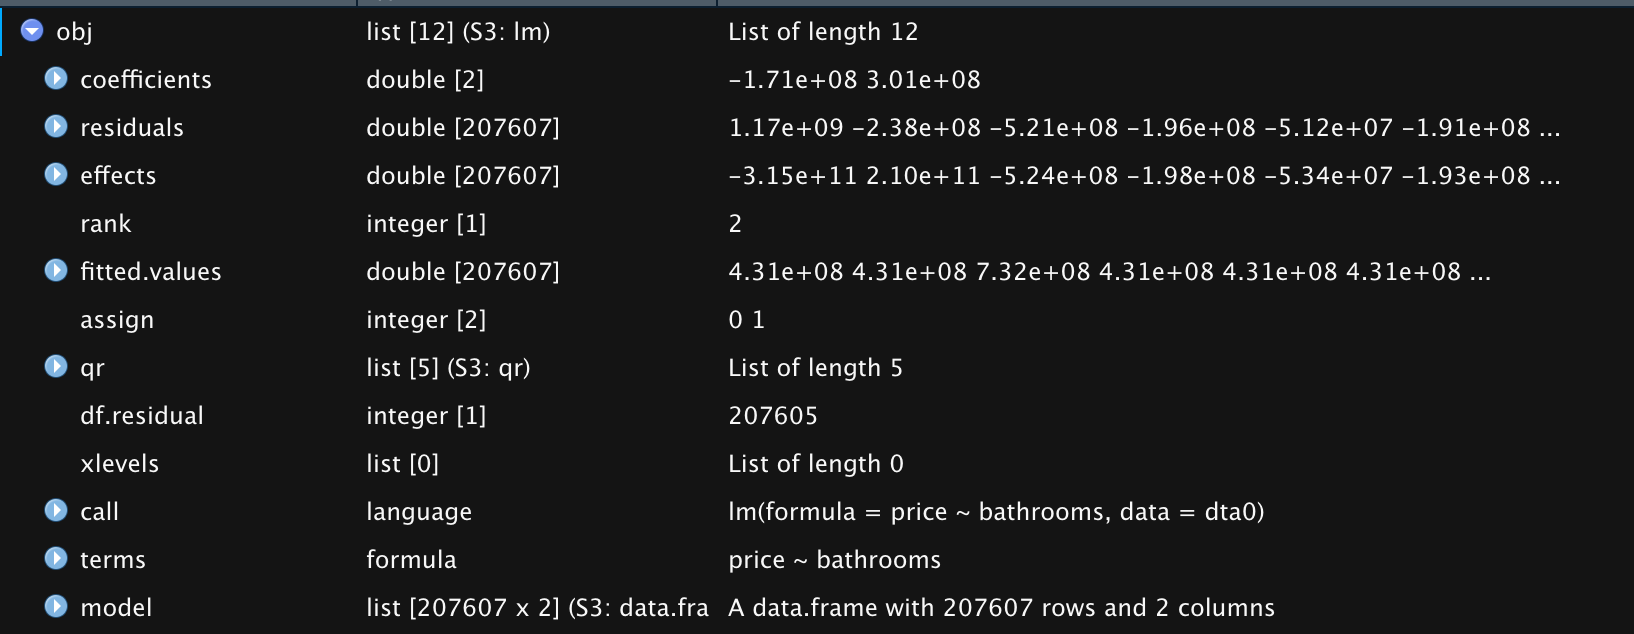
\includegraphics[scale=0.45]{figures/lm_object.png}
  \\
  \tiny 
\end{figure}


Note that \texttt{R's} \texttt{lm} also returns many objects that have the same size as X and Y

\end{frame}



%----------------------------------------------------------------------%
\subsection{Gradient-Based Optimization}
%----------------------------------------------------------------------%
\begin{frame}[fragile]
\frametitle{Gradient-Based Optimization}


\begin{itemize}
\item Suppose we have a function $y=f(x)$, where both x and y are real numbers.

\item The derivative $f'(x)$ gives the slope of $f(x)$ at the point x
\item  It specifies how to scale a small change in the input to obtain the corresponding change in the output

\begin{align}
f(x+\epsilon)\approx f(x)+\epsilon f'(x)
\end{align}

\item The derivative is therefore useful for minimizing a function because it tells us how to change x
in order to make a small improvement in y
\item  We can thus reduce $f(x)$ by moving x in small steps with the opposite sign of the derivative.
\item This technique is called gradient descent (Cauchy, 1847).

\end{itemize}

\end{frame}
%----------------------------------------------------------------------%
\begin{frame}[fragile]
\frametitle{Gradient-Based Optimization}



\begin{figure}[H] \centering
            \captionsetup{justification=centering}
              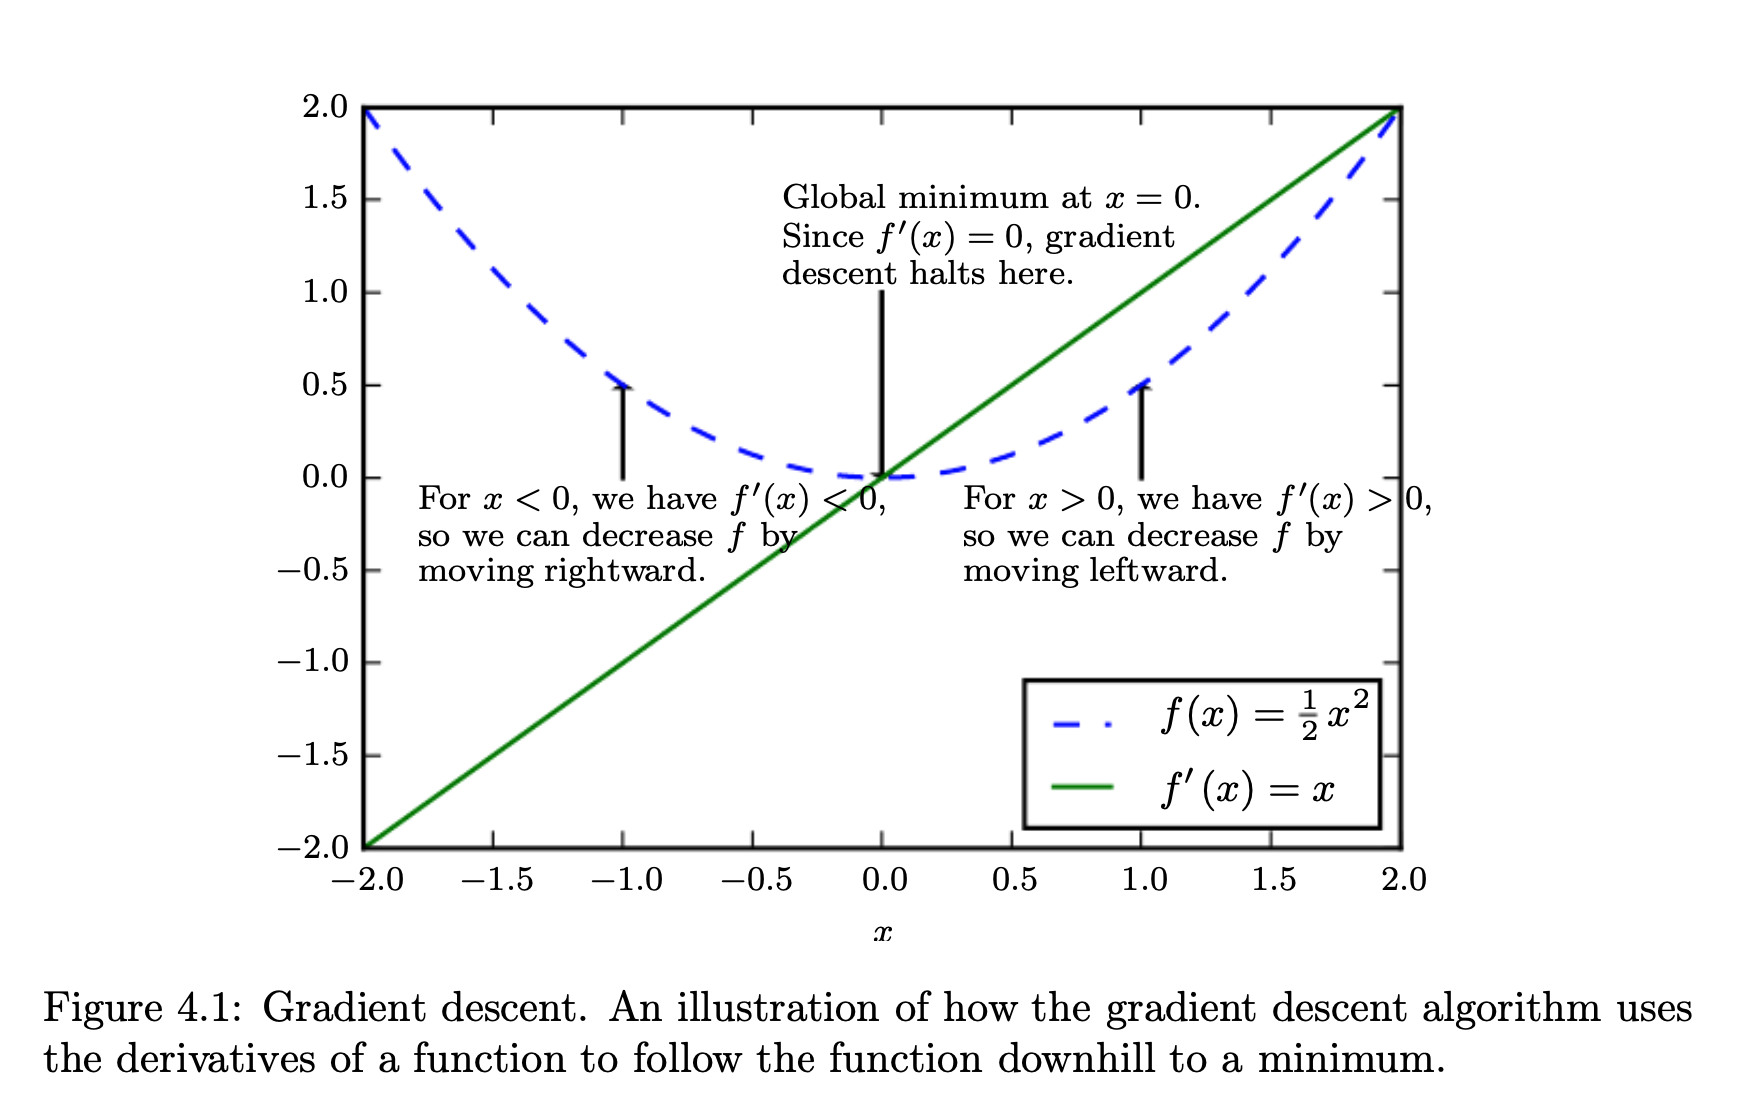
\includegraphics[scale=0.4]{figures/gradient_descent}
 \end{figure}
 \end{frame}
 %----------------------------------------------------------------------%
\begin{frame}[fragile]
\frametitle{Gradient-Based Optimization}



\begin{figure}[H] \centering
            \captionsetup{justification=centering}
              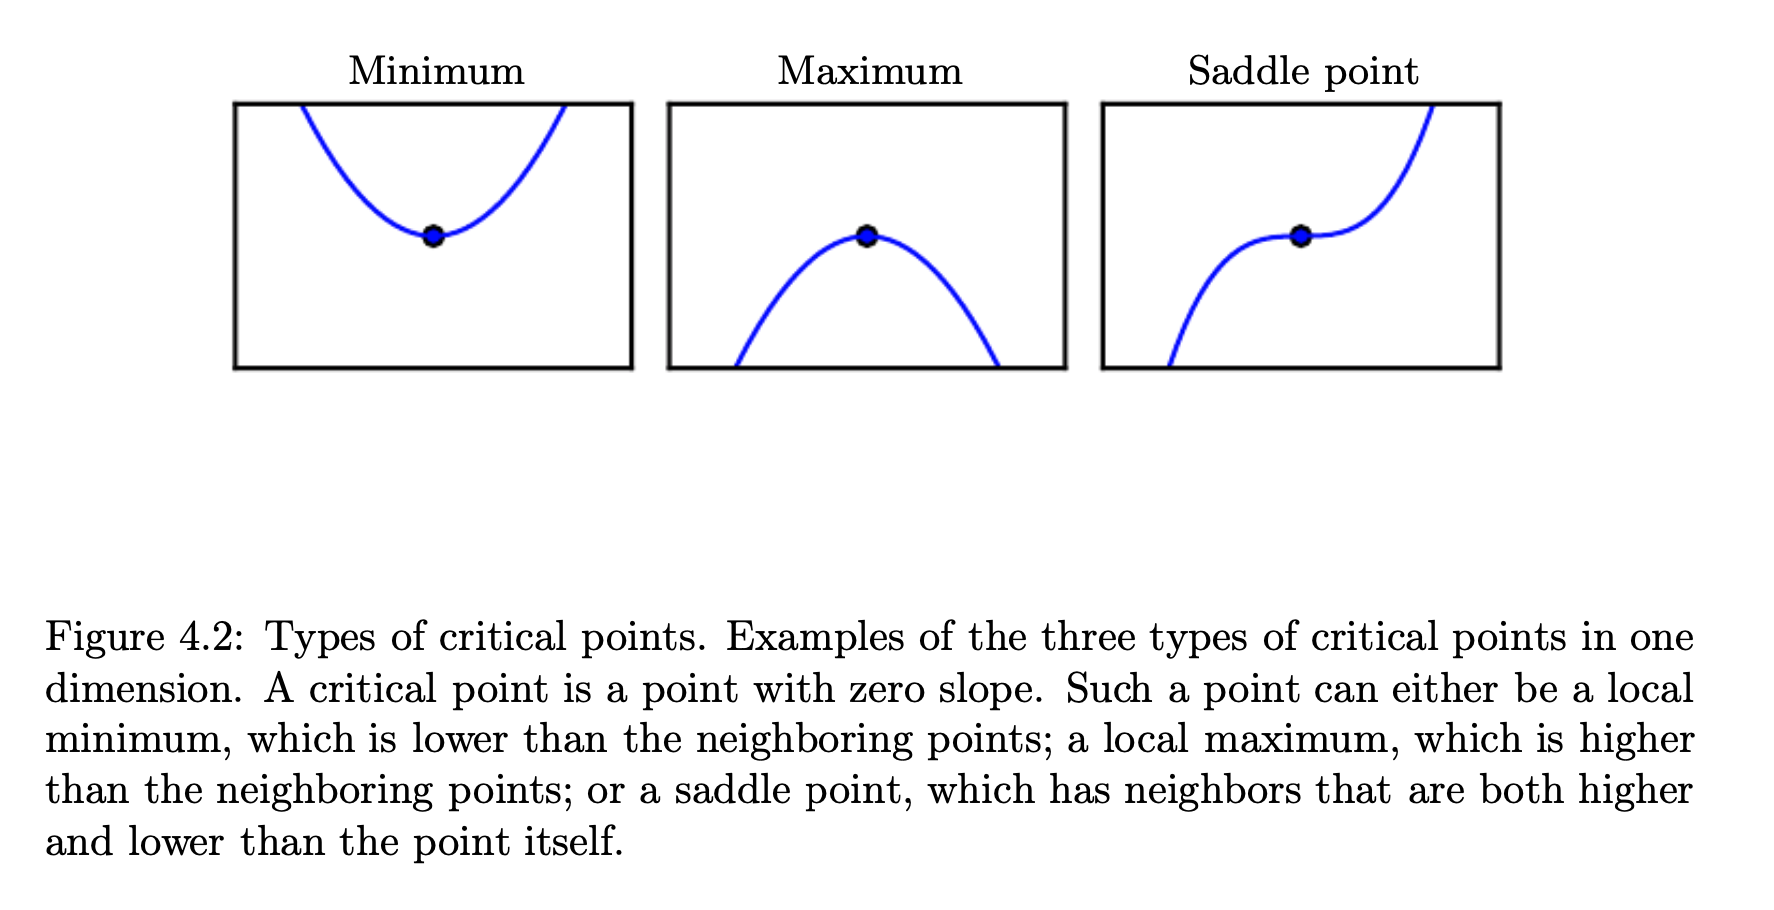
\includegraphics[scale=0.4]{figures/gradient_descent_2}
 \end{figure}
 
 \end{frame}
%----------------------------------------------------------------------%
\begin{frame}[fragile]
\frametitle{Gradient-Based Optimization}



\begin{figure}[H] \centering
            \captionsetup{justification=centering}
              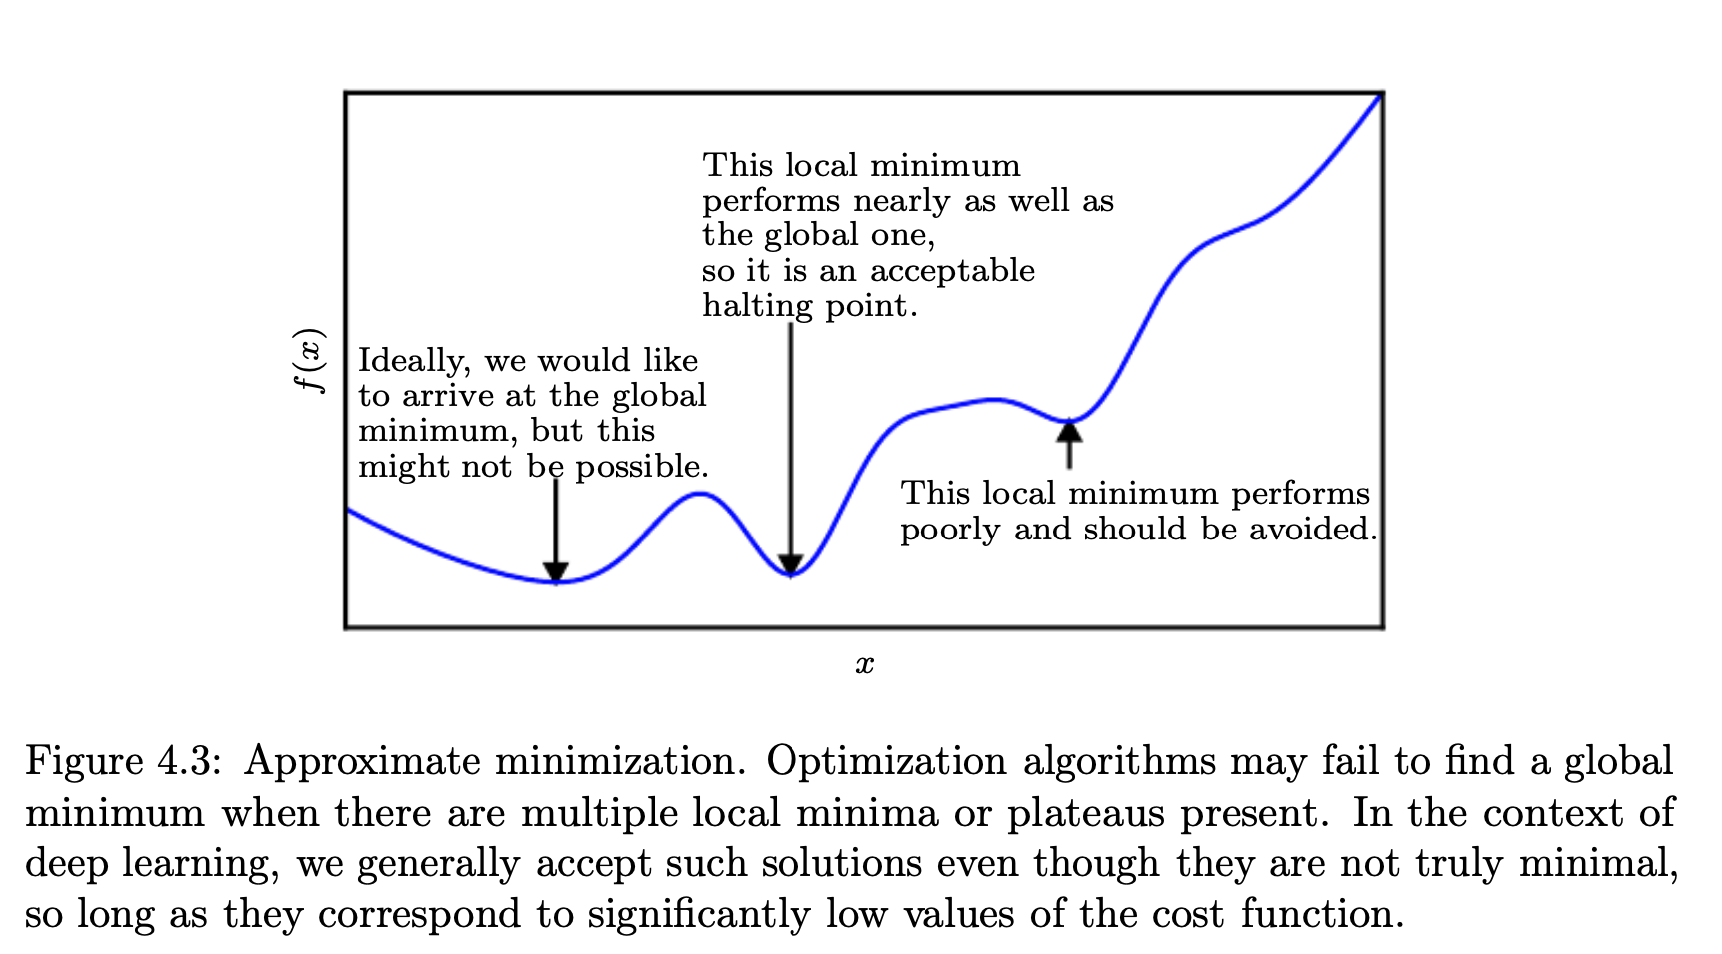
\includegraphics[scale=0.4]{figures/gradient_descent_3}
 \end{figure}
 
  \end{frame}
\begin{comment}
  
%----------------------------------------------------------------------%
\begin{frame}[fragile]
\frametitle{Gradient-Based Optimization}

\begin{itemize}


\item The directional derivative in direction $\mathbf{u}$ (a unit vector) is the slope of the function $f$ in direction $\mathbf{u}$. 
\item In other words, the directional derivative is the derivative of 
\begin{align}
f(x+\alpha u)
\end{align}
\item with respect to $\alpha$, evaluated at $\alpha=0$
\begin{align}
\frac{\partial}{\partial \alpha} = \mathbf{u}'\nabla_x f(\mathbf{u}) 
\end{align}
\end{itemize}

 
  \end{frame}
%----------------------------------------------------------------------%
\begin{frame}[fragile]
\frametitle{Gradient-Based Optimization}

\begin{itemize}
\item To minimize $f$, we would like to find the direction in which f decreases the fastest. 
\item We can use the directional derivative:

\begin{align}
\underset{u,u'u=1}{min}\mathbf{u}'\nabla_x f(\mathbf{u}) 
\end{align}
\begin{align}
\underset{u,u'u=1}{min}||\mathbf{u}||_2||\nabla_x f(\mathbf{u})||_2 \cos\,\theta 
\end{align}

\item Where $\theta$ is the angle between $\mathbf{u}$ and the gradient.  Substituting $u'u=1$ 

\begin{align}
\underset{u,u'u=1}{min} \cos\,\theta 
\end{align}

\item This is minimized when $\mathbf{u}$ points in the opposite direction as the gradient.
\item In other words, the gradient points directly uphill, and the negative gradient points directly downhill.
\item We can decrease $f$ by moving in the direction of the negative gradient.


\end{itemize}

 
  \end{frame}
\end{comment}
%----------------------------------------------------------------------%
\begin{frame}[fragile]
\frametitle{Gradient-Based Optimization}

\begin{itemize}
  \item {\bf Steepest descent}, or {\bf gradient descent} proposes a new point

    \begin{align}
    \theta'=\theta-\epsilon \nabla_\theta f(\theta)
    \end{align}
\item where $\epsilon$ is the learning rate, a positive scalar determining the size of the step. 

\end{itemize}




\begin{figure}[H] \centering
  \centering
  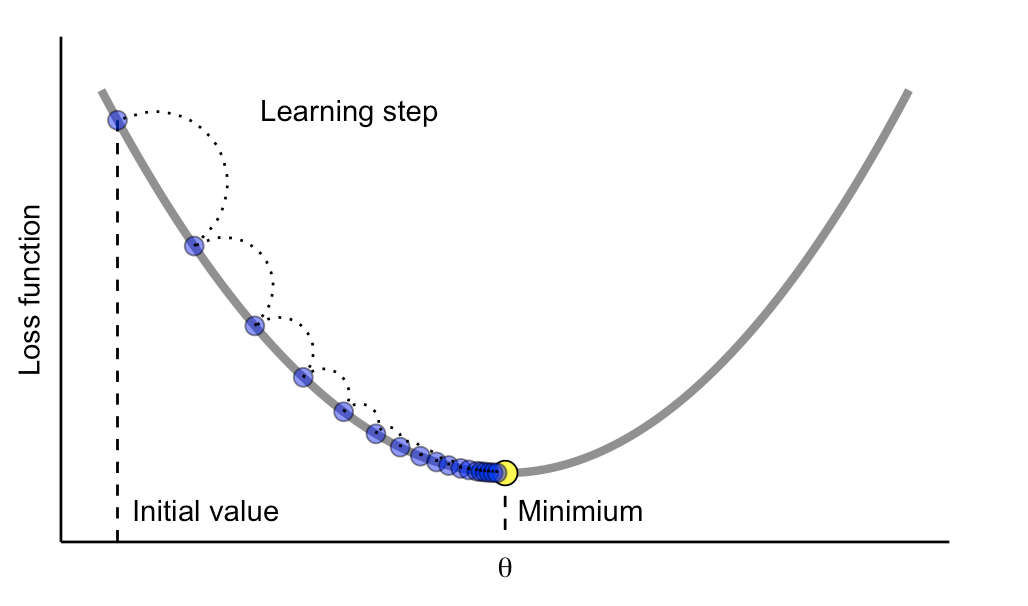
\includegraphics[scale=0.25]{figures/step_size1.png}
  \\
  \tiny
  Source: Boehmke, B., \& Greenwell, B. (2019)
\end{figure}
 
  \end{frame}
%----------------------------------------------------------------------%
\begin{frame}[fragile]
\frametitle{Gradient-Based Optimization}


\begin{figure}[H] \centering
  \centering
  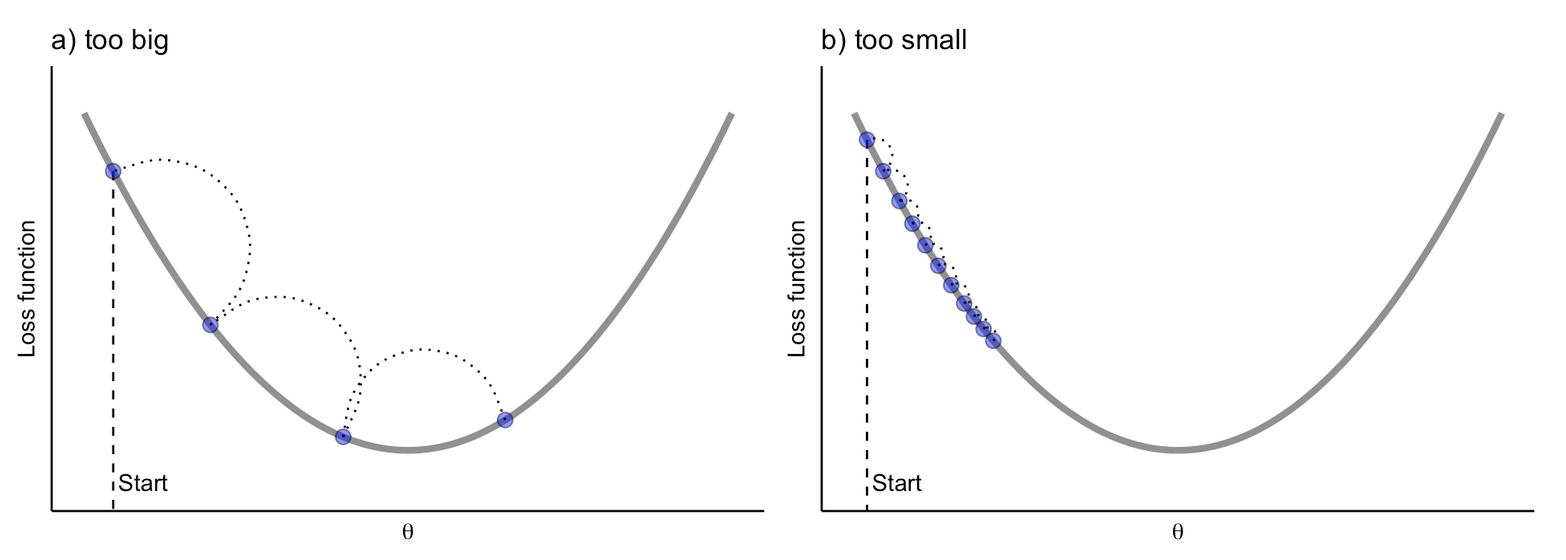
\includegraphics[scale=0.3]{figures/step_size2.png}
  \\
  \tiny
  Source: Boehmke, B., \& Greenwell, B. (2019)
\end{figure}

\begin{itemize}
  \footnotesize
\item We can choose $\epsilon$ in several different ways:
\begin{itemize}
  \tiny
\item A popular approach is to set $\epsilon$ to a small constant. 
 \item Sometimes, we can solve for the step size that makes the directional derivative vanish. 
 \item Another approach is to evaluate $f(\theta-\epsilon \nabla_\theta f(\theta))$ for several values of 
 $\epsilon$ and choose the one that results in the smallest objective function value. This  is called a line search.
\end{itemize}
 

\item Steepest descent converges when every element of the gradient is zero (or, in practice, very close to zero). 
\item In some cases, we may be able to avoid running this iterative algorithm and just jump directly to the critical point by solving the equation $\nabla_\theta f(\theta)=0$ for x.

\end{itemize}




 \end{frame}
%----------------------------------------------------------------------%
\begin{frame}[fragile]
\frametitle{Gradient-Based Optimization}





\begin{minipage}[c]{0.38\linewidth}
        
\begin{table}[]
\begin{tabular}{cc}
log(wage) & Education (years) \\
5         & 8                                                         \\
10        & 12                                                          \\
12.5      & 16                                                          \\
\end{tabular}
\end{table}
           
    \end{minipage}
    \hfill
    \begin{minipage}[t]{0.58\linewidth}%
        \begin{figure}[H] \centering
            \captionsetup{justification=centering}  
            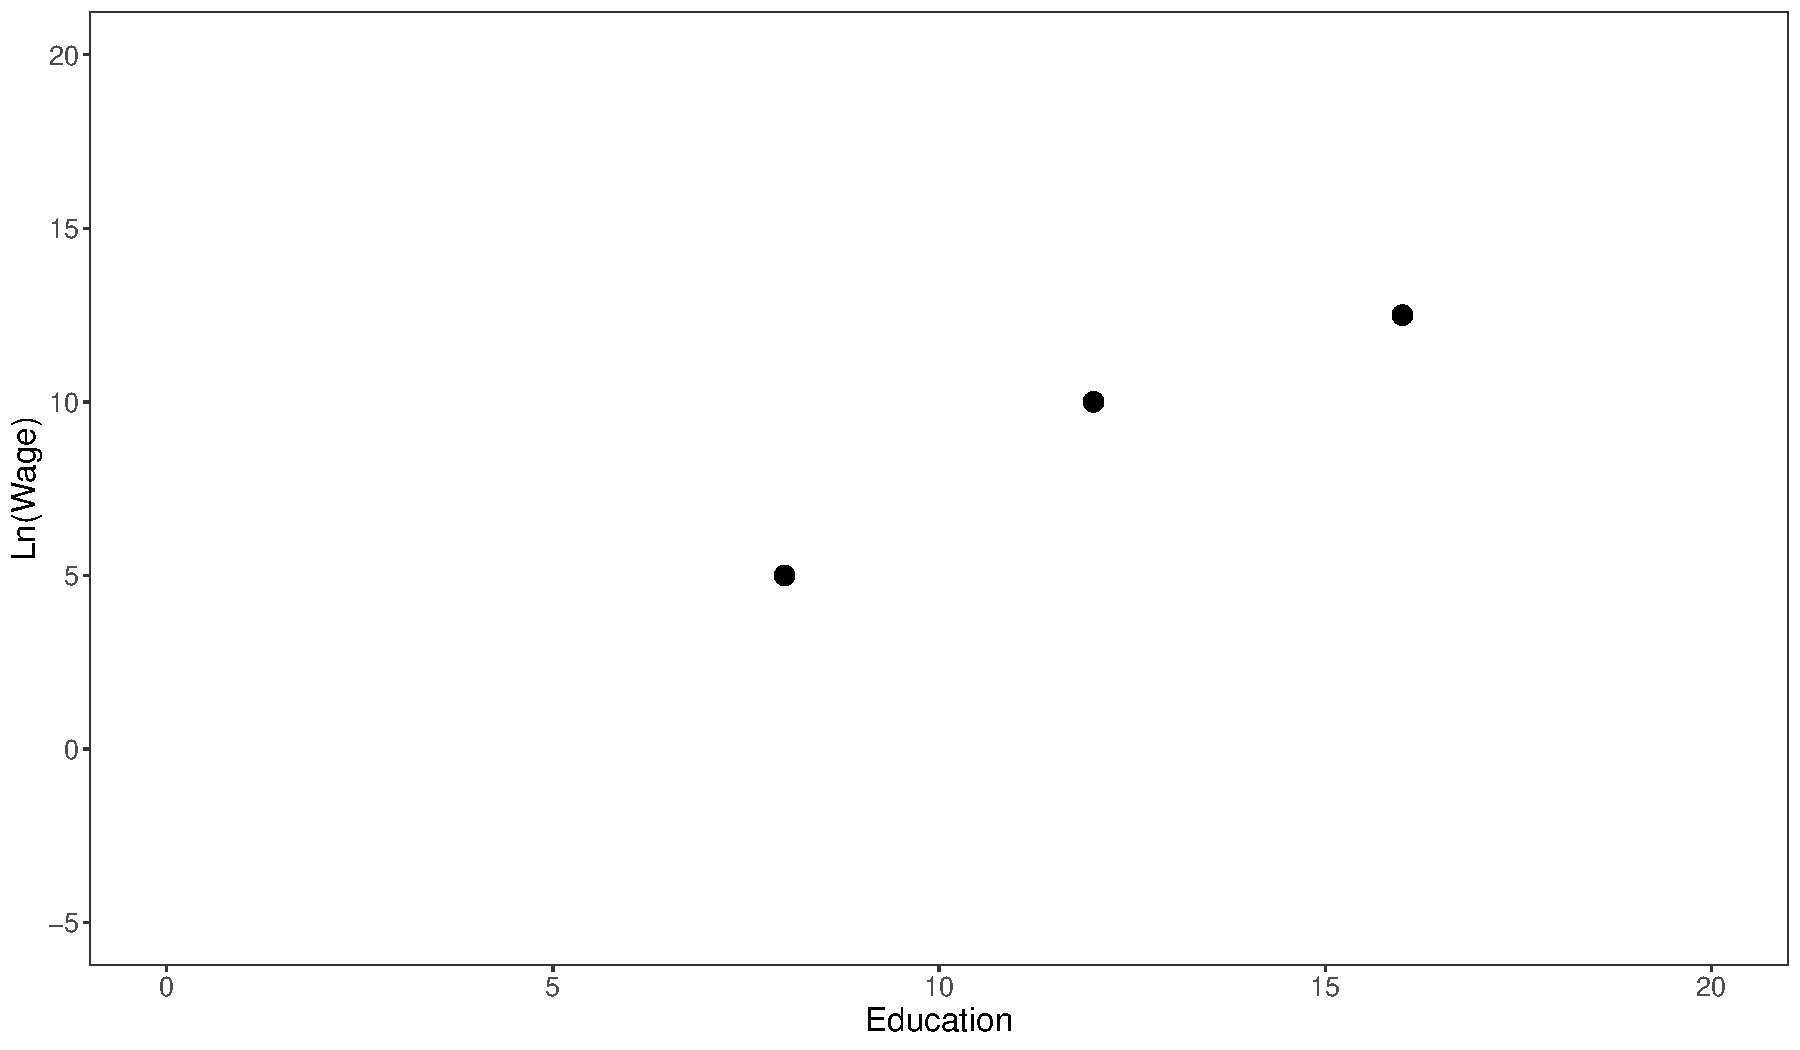
\includegraphics[scale=0.25]{figures/fig_1.pdf}
    \end{figure}
    \end{minipage}

\end{frame}
%----------------------------------------------------------------------%
\begin{frame}[fragile]
\frametitle{Gradient-Based Optimization}





\begin{minipage}[c]{0.38\linewidth}
        
\begin{table}[]
\begin{tabular}{cc}
log(wage) & Education (years) \\
5         & 8                                                         \\
10        & 12                                                          \\
12.5      & 16                                                          \\
\end{tabular}
\end{table}

\bigskip

\begin{align}
\hat \beta=(X'X)^{-1}X'y \nonumber
\end{align}




\begin{Shaded}
%\begin{Highlighting}[]
\begin{verbatim}
beta<-solve(t(X)%*%X)%*%t(X)%*%y

lm(y~x,data)
\end{verbatim}
%\end{Highlighting}
\end{Shaded}

\begin{align}
y=-2.0833 +  0.9375 \times Educ \nonumber
\end{align}

    \end{minipage}
    \hfill
    \begin{minipage}[c]{0.58\linewidth}%
        \begin{figure}[H] \centering
            \captionsetup{justification=centering}  
            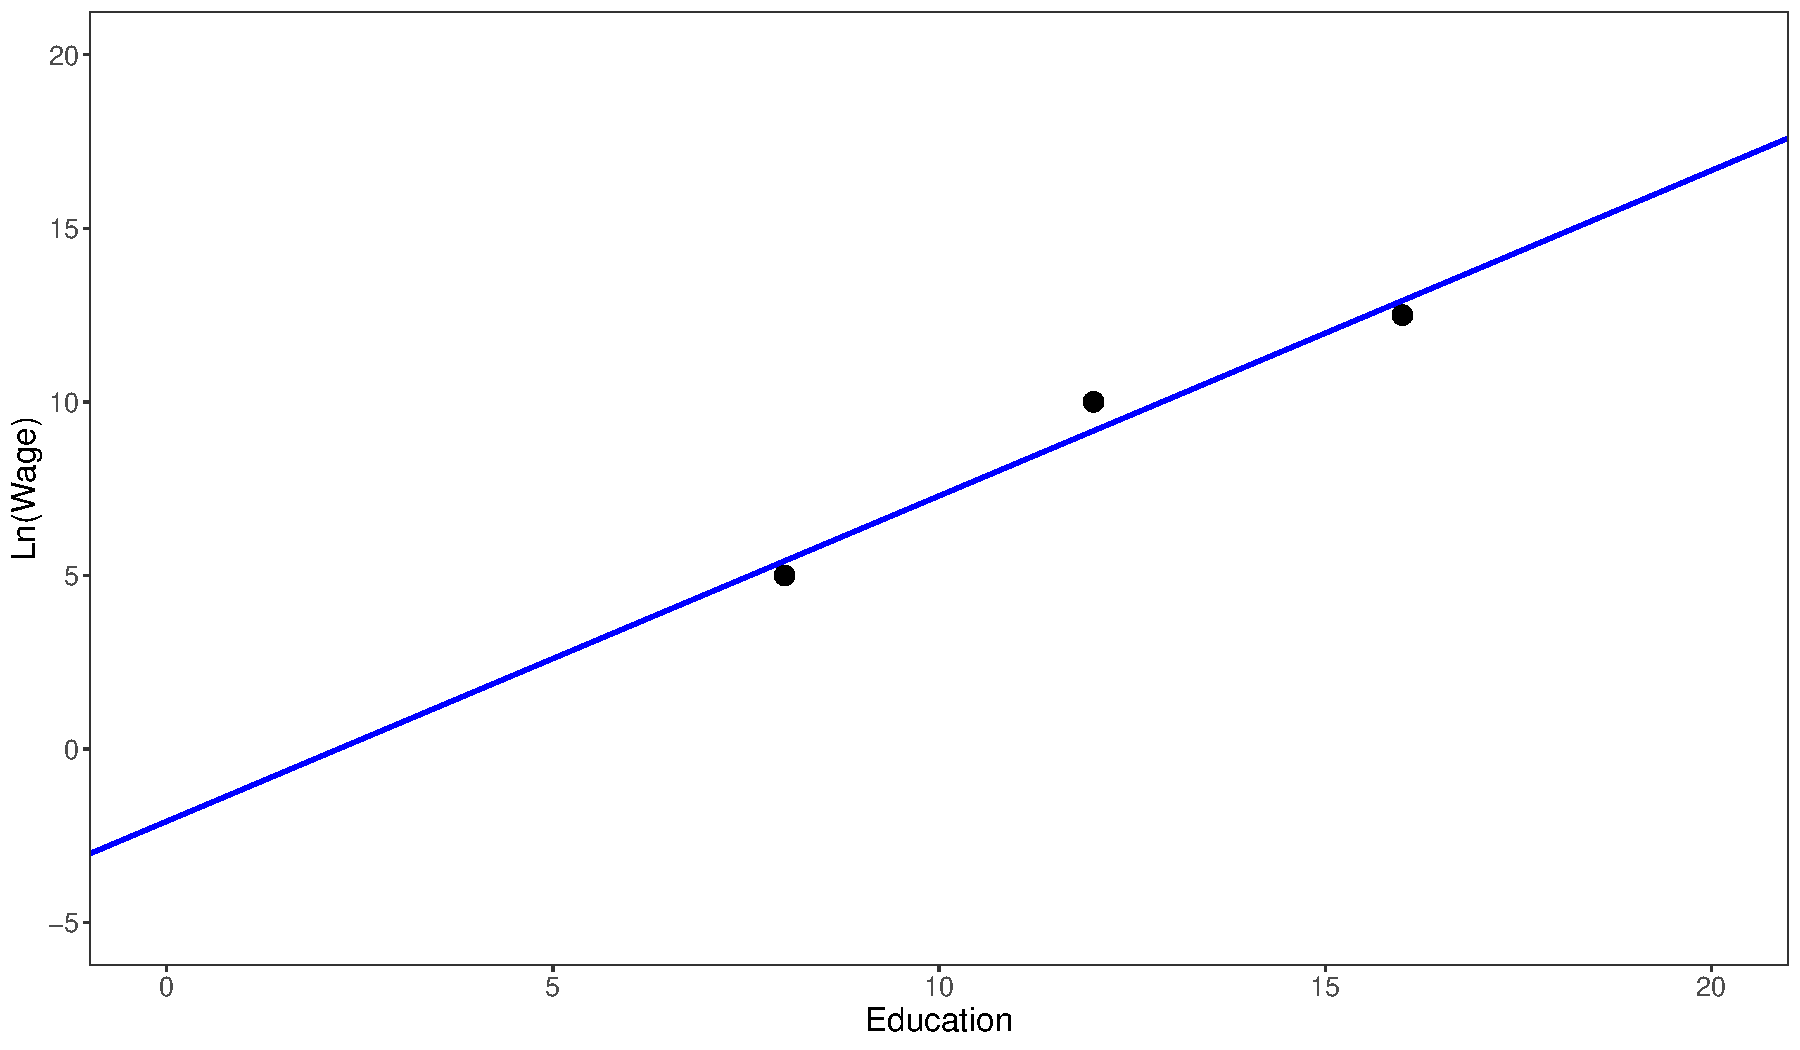
\includegraphics[scale=0.25]{figures/fig_1b.pdf}
    \end{figure}
    \end{minipage}

\end{frame}
%----------------------------------------------------------------------%
\begin{frame}[fragile]
\frametitle{Gradient-Based Optimization}






The Loss Function         
\begin{align}
SSR=f(\theta)=\sum_{i=1}^{n}(y_{i}-(\alpha+\beta x_{i}))^{2} \nonumber
\end{align}

The Gradient

\begin{align}
\nabla f_{\theta}(\theta)=\left(\begin{array}{c}
\frac{\partial f}{\partial\alpha}\\
\frac{\partial f}{\partial\beta}
\end{array}\right)=\left(\begin{array}{c}
-2\sum_{i=1}^{n}(y_{i}-\alpha-\beta x_{i})\\
-2\sum_{i=1}^{n}x_{i}(y_{i}-\alpha-\beta x_{i})
\end{array}\right)  \nonumber
\end{align}

Updating
\begin{align}
\alpha' &=\alpha-\epsilon\frac{\partial f}{\partial\alpha} \nonumber \\
\beta' &= \beta-\epsilon\frac{\partial f}{\partial\beta} \nonumber
\end{align}

\end{frame}
%----------------------------------------------------------------------%
\begin{frame}[fragile]
\frametitle{Gradient-Based Optimization}
\tiny
First Iteration
\begin{table}[]
\begin{tabular}{cc}
log(wage) & Education (years) \\
5         & 8                                                         \\
10        & 12                                                          \\
12.5      & 16                                                          \\
\end{tabular}
\end{table}

Start with an initial guess: $\alpha=-1;\beta=2$ , and a learning rate ($\epsilon=0.005$). Then we have

\begin{align}
\alpha' &=(-1)-0.005\left(-2\left((5-(-1)-2\times8)+(10-(-1)-2\times12\right)+(12.5-(-1)-2\times16)\right) \nonumber \\
\beta' &=2+0.005\left(-2\left(8(5-(-1)-2\times8)+12(10-(-1)-2\times12\right)+16(12.5-(-1)-2\times16)\right) \nonumber \\
\alpha'&=-1.1384 \nonumber \\
\beta' &=0.2266 \nonumber
\end{align}





    
        \begin{figure}[H] \centering
            \captionsetup{justification=centering}  
            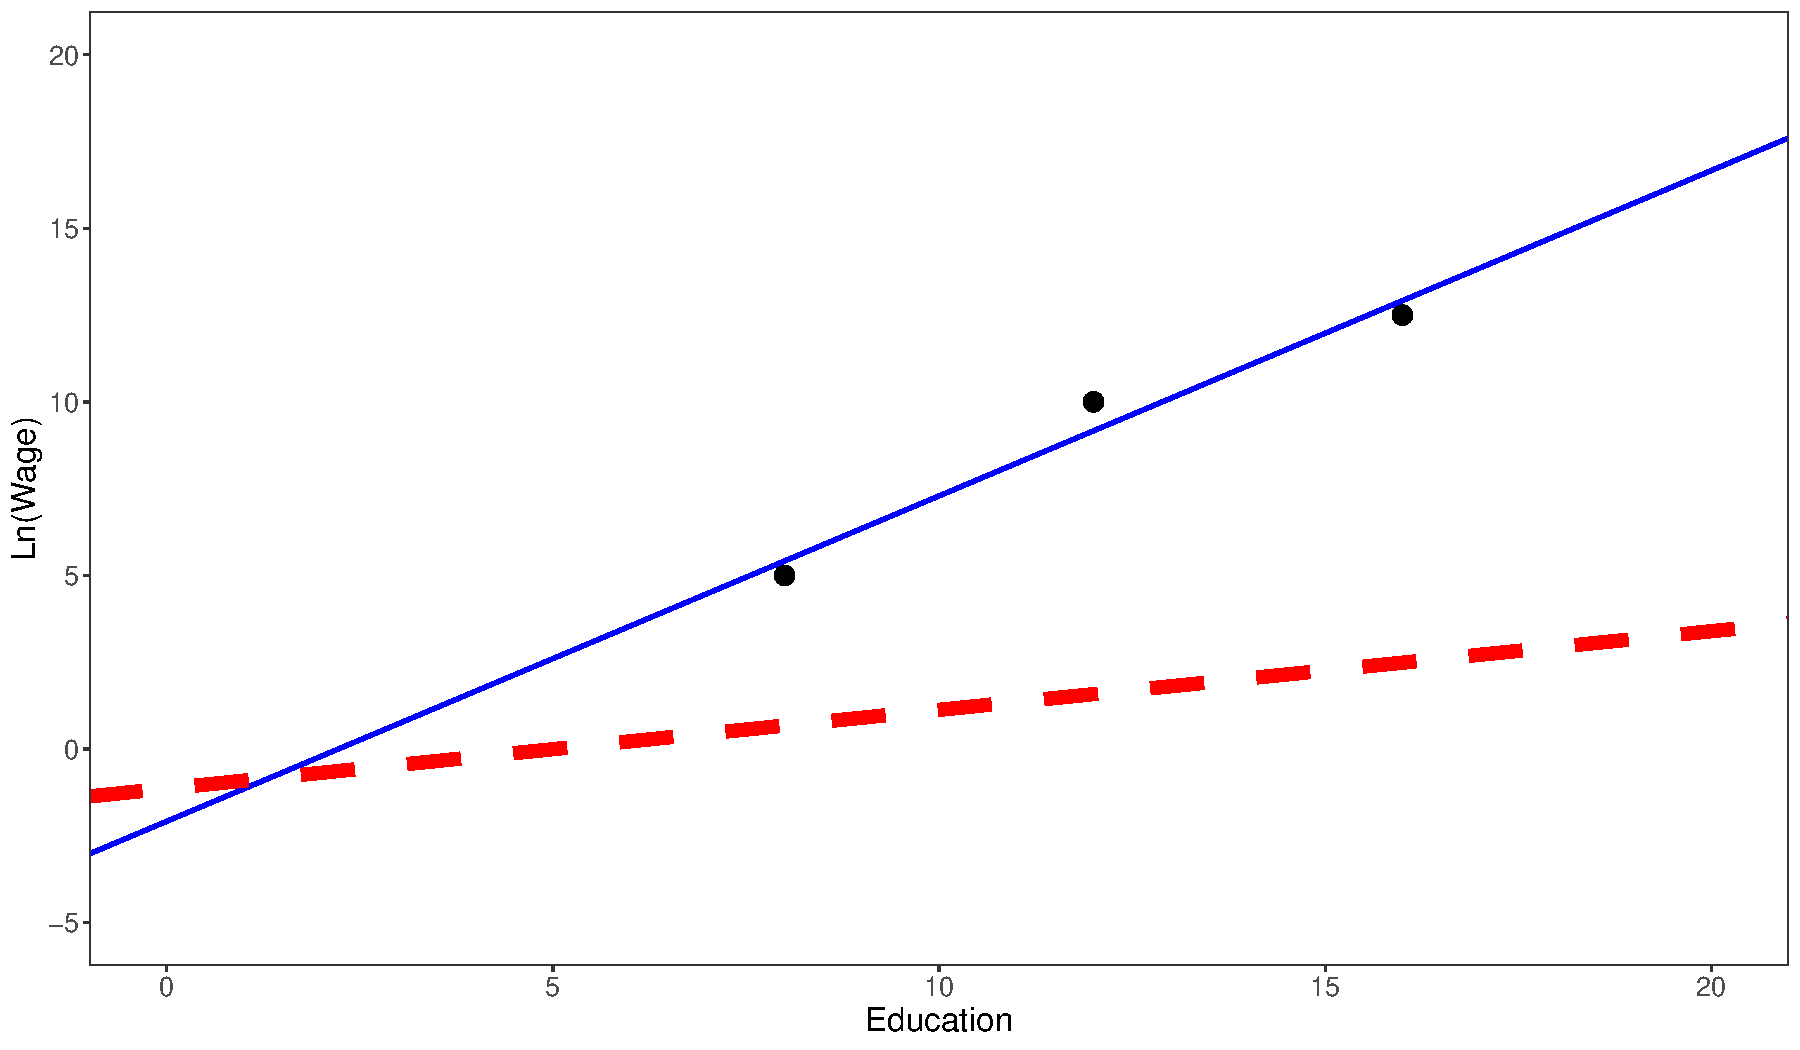
\includegraphics[scale=0.15]{figures/fig_1_2.pdf}
    \end{figure}




\end{frame}
%----------------------------------------------------------------------%
\begin{frame}[fragile]
\frametitle{Gradient-Based Optimization}
\tiny
Second Iteration
\begin{table}[]
\begin{tabular}{cc}
log(wage) & Education (years) \\
5         & 8                                                         \\
10        & 12                                                          \\
12.5      & 16                                                          \\
\end{tabular}
\end{table}

Start with an initial guess: $\alpha=-1;\beta=2$ , and a learning rate ($\epsilon=0.005$). Then we have

\begin{align}
\alpha^2 &=(-1.1384)-0.005\left(-2\left((5-(-1.1384)-(0.2266)\times8)+(10-(-1.1384)-(0.2266)\times12\right)+(12.5-(-1.1384)-(0.2266)\times16)\right) \nonumber \\
\beta^2 &=(0.2266)+0.005\left(-2\left(8(5-(-1.1384)-(0.2266)\times8)+12(10-(-1.1384)-(0.2266)\times12\right)+16(12.5-(-1.1384)-(0.2266)\times16)\right) \nonumber \\
\alpha^2&= -1.0624 \nonumber \\
\beta^2 &= 1.212689 \nonumber
\end{align}





    
        \begin{figure}[H] \centering
            \captionsetup{justification=centering}  
            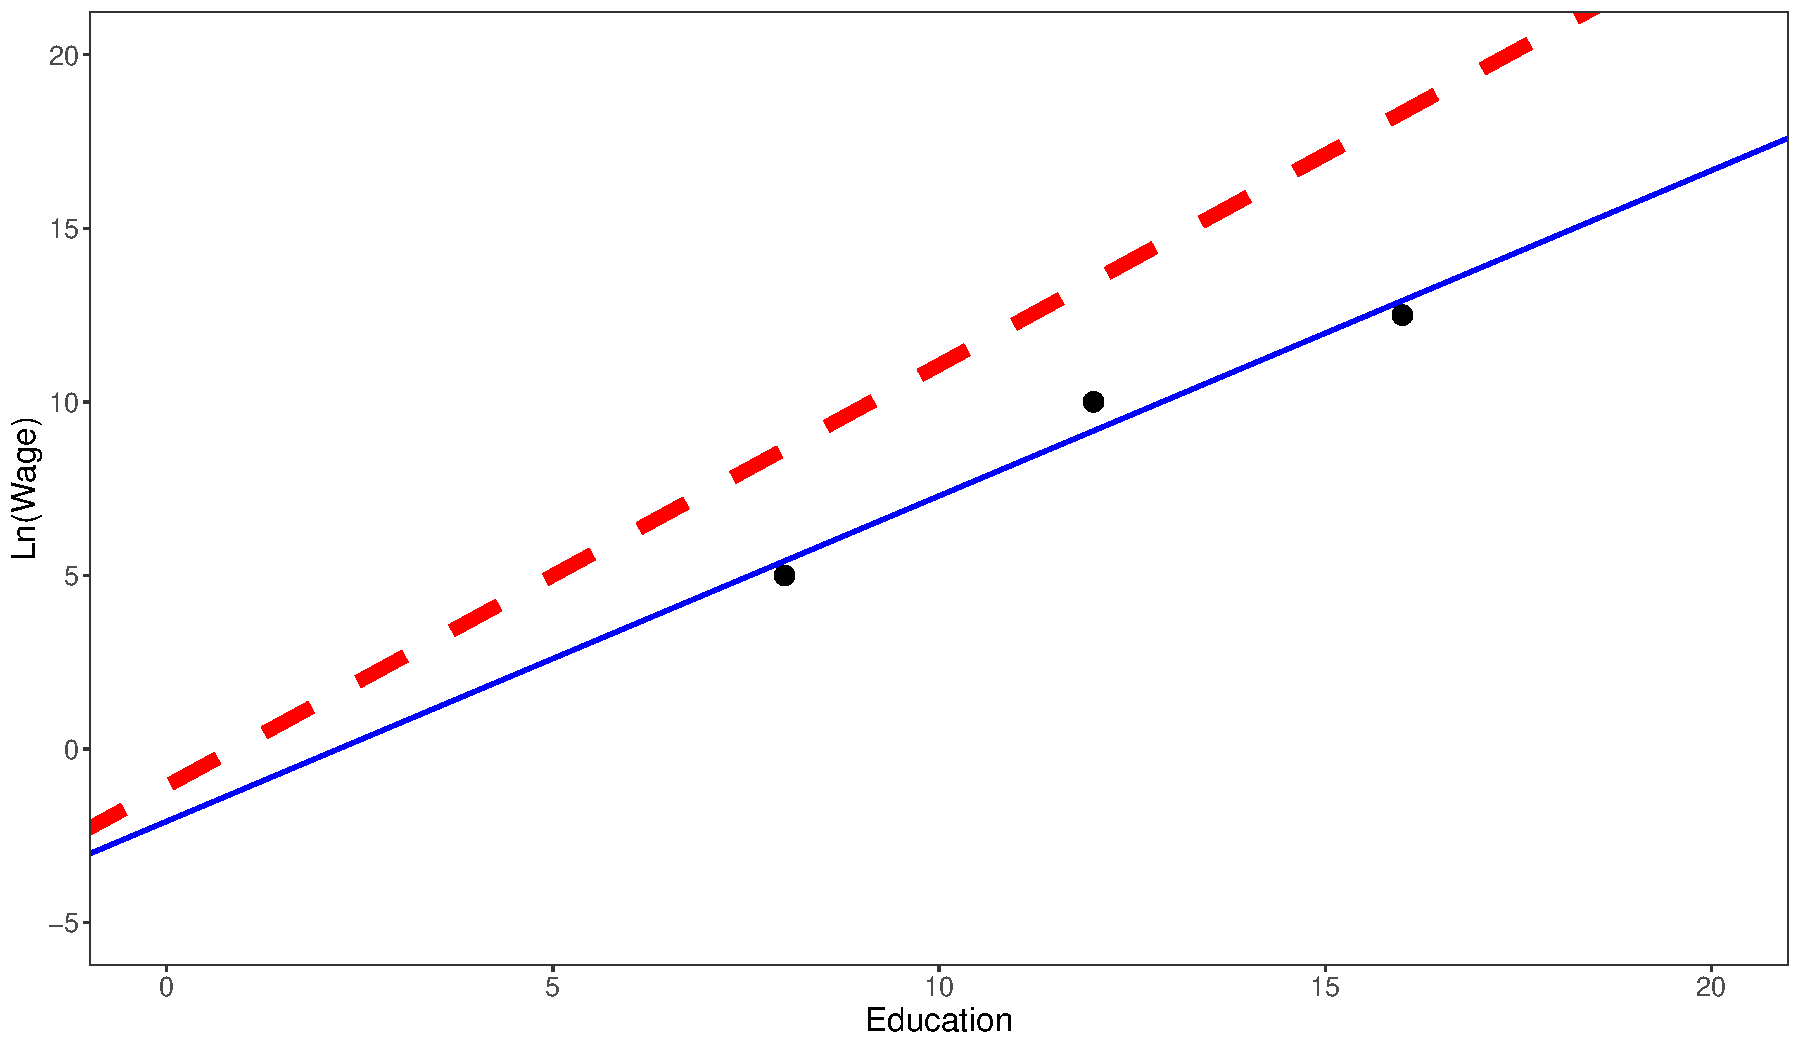
\includegraphics[scale=0.15]{figures/fig_1_3.pdf}
    \end{figure}



\end{frame}
%----------------------------------------------------------------------%
\begin{frame}[fragile]
\frametitle{Gradient-Based Optimization}
\tiny
Third Iteration
\begin{table}[]
\begin{tabular}{cc}
log(wage) & Education (years) \\
5         & 8                                                         \\
10        & 12                                                          \\
12.5      & 16                                                          \\
\end{tabular}
\end{table}



\begin{align}
\alpha^3&= -1.0624 \nonumber \\
\beta^3 &= 1.212689 \nonumber
\end{align}





    
        \begin{figure}[H] \centering
            \captionsetup{justification=centering}  
            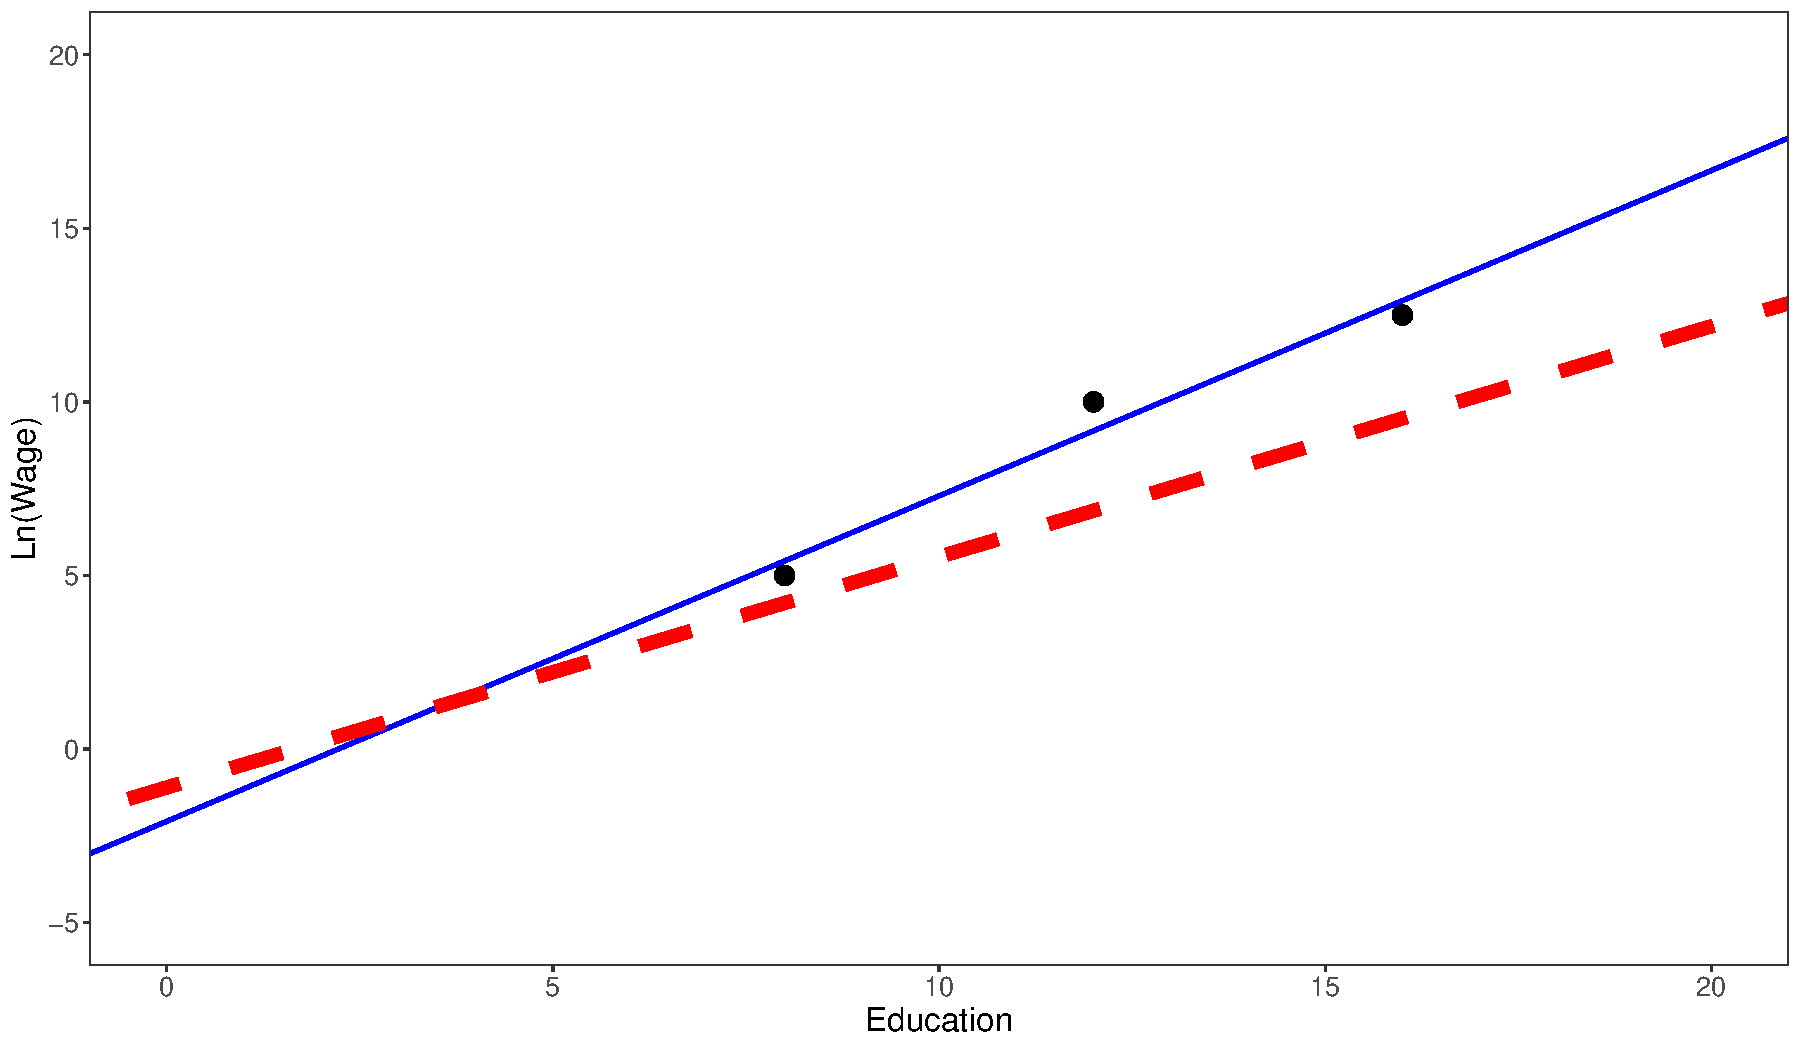
\includegraphics[scale=0.15]{figures/fig_1_4.pdf}
    \end{figure}


\end{frame}
%----------------------------------------------------------------------%
\begin{frame}[fragile]
\frametitle{Gradient-Based Optimization}
\tiny
Fourth Iteration
\begin{table}[]
\begin{tabular}{cc}
log(wage) & Education (years) \\
5         & 8                                                         \\
10        & 12                                                          \\
12.5      & 16                                                          \\
\end{tabular}
\end{table}



\begin{align}
\alpha^4&=  -1.082738 \nonumber \\
\beta^4 &= 0.9693922 \nonumber
\end{align}


        \begin{figure}[H] \centering
            \captionsetup{justification=centering}  
            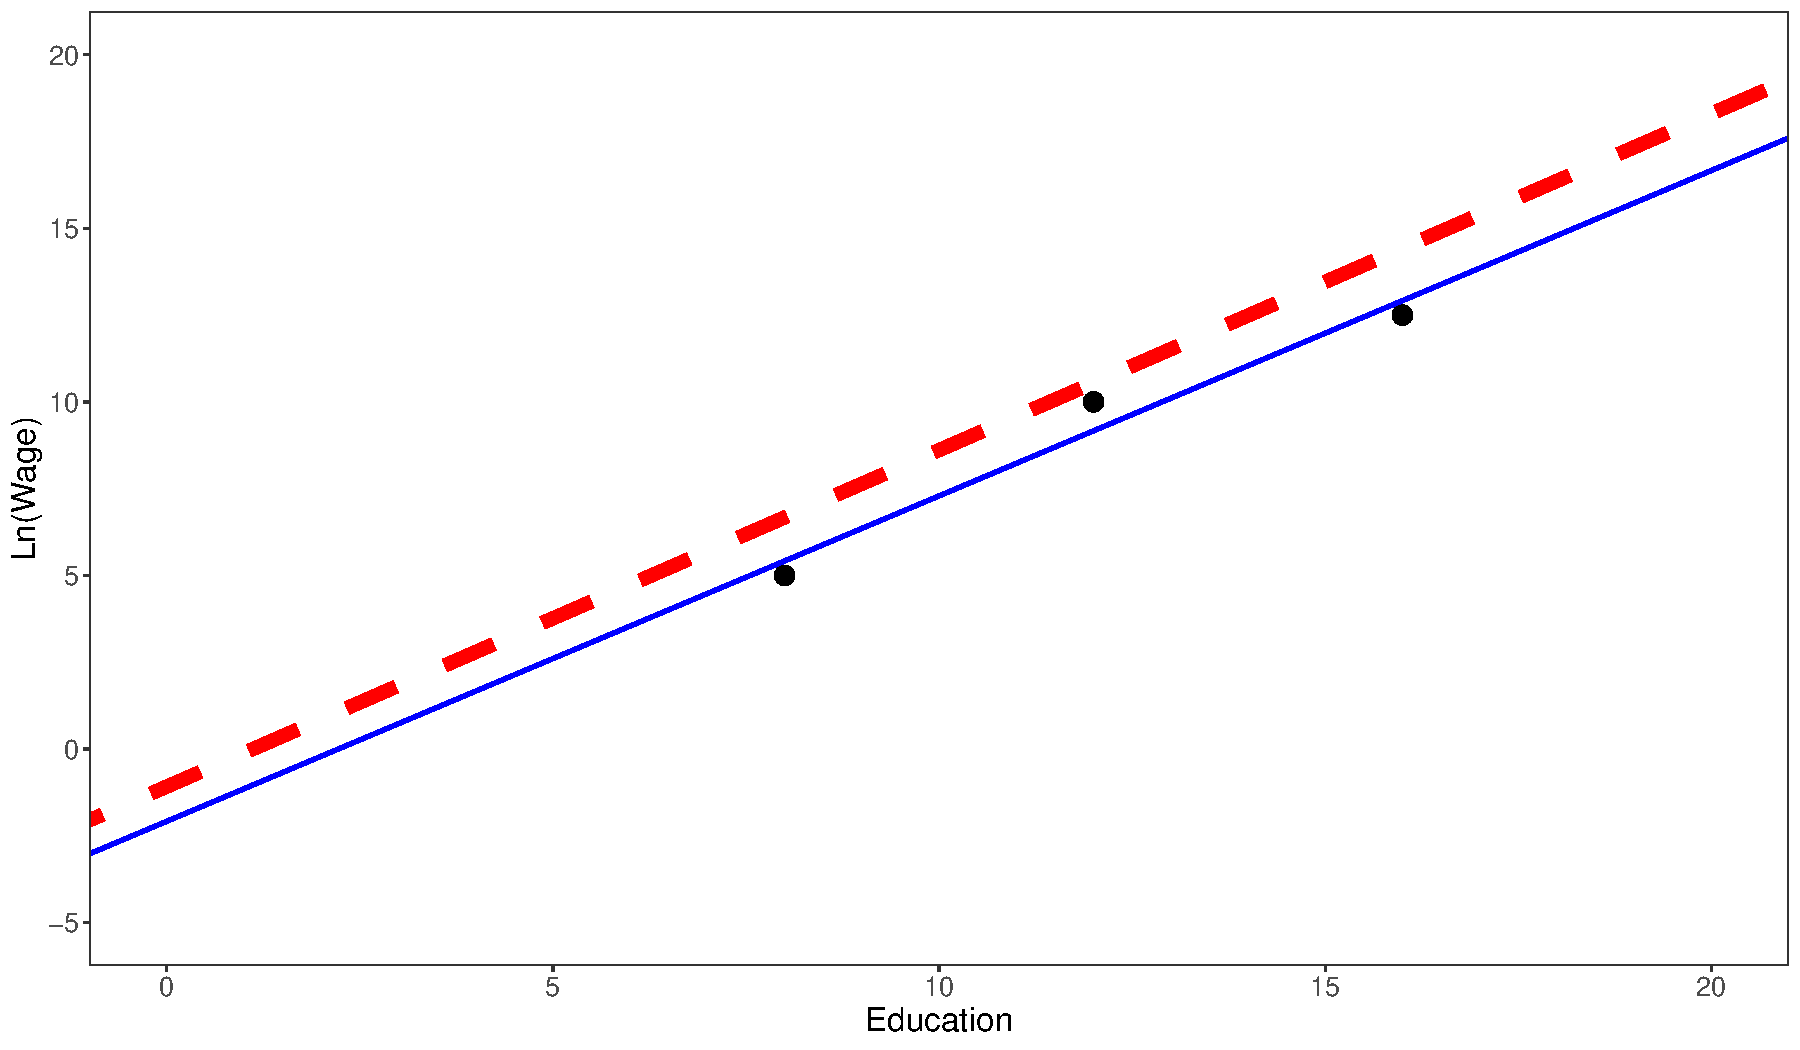
\includegraphics[scale=0.15]{figures/fig_1_5.pdf}
    \end{figure}



\end{frame}
%----------------------------------------------------------------------%
\begin{frame}[fragile]
\frametitle{Gradient-Based Optimization}
\tiny
7211 Iteration
\begin{table}[]
\begin{tabular}{cc}
log(wage) & Education (years) \\
5         & 8                                                         \\
10        & 12                                                          \\
12.5      & 16                                                          \\
\end{tabular}
\end{table}



\begin{align}
\alpha^{7211} &=  -2.076246 \nonumber \\
\beta^{7211} &=  0.9369499 \nonumber
\end{align}


\begin{align}
y^{ols}=-2.0833 +  0.9375 \times Educ \nonumber
\end{align}


        \begin{figure}[H] \centering
            \captionsetup{justification=centering}  
            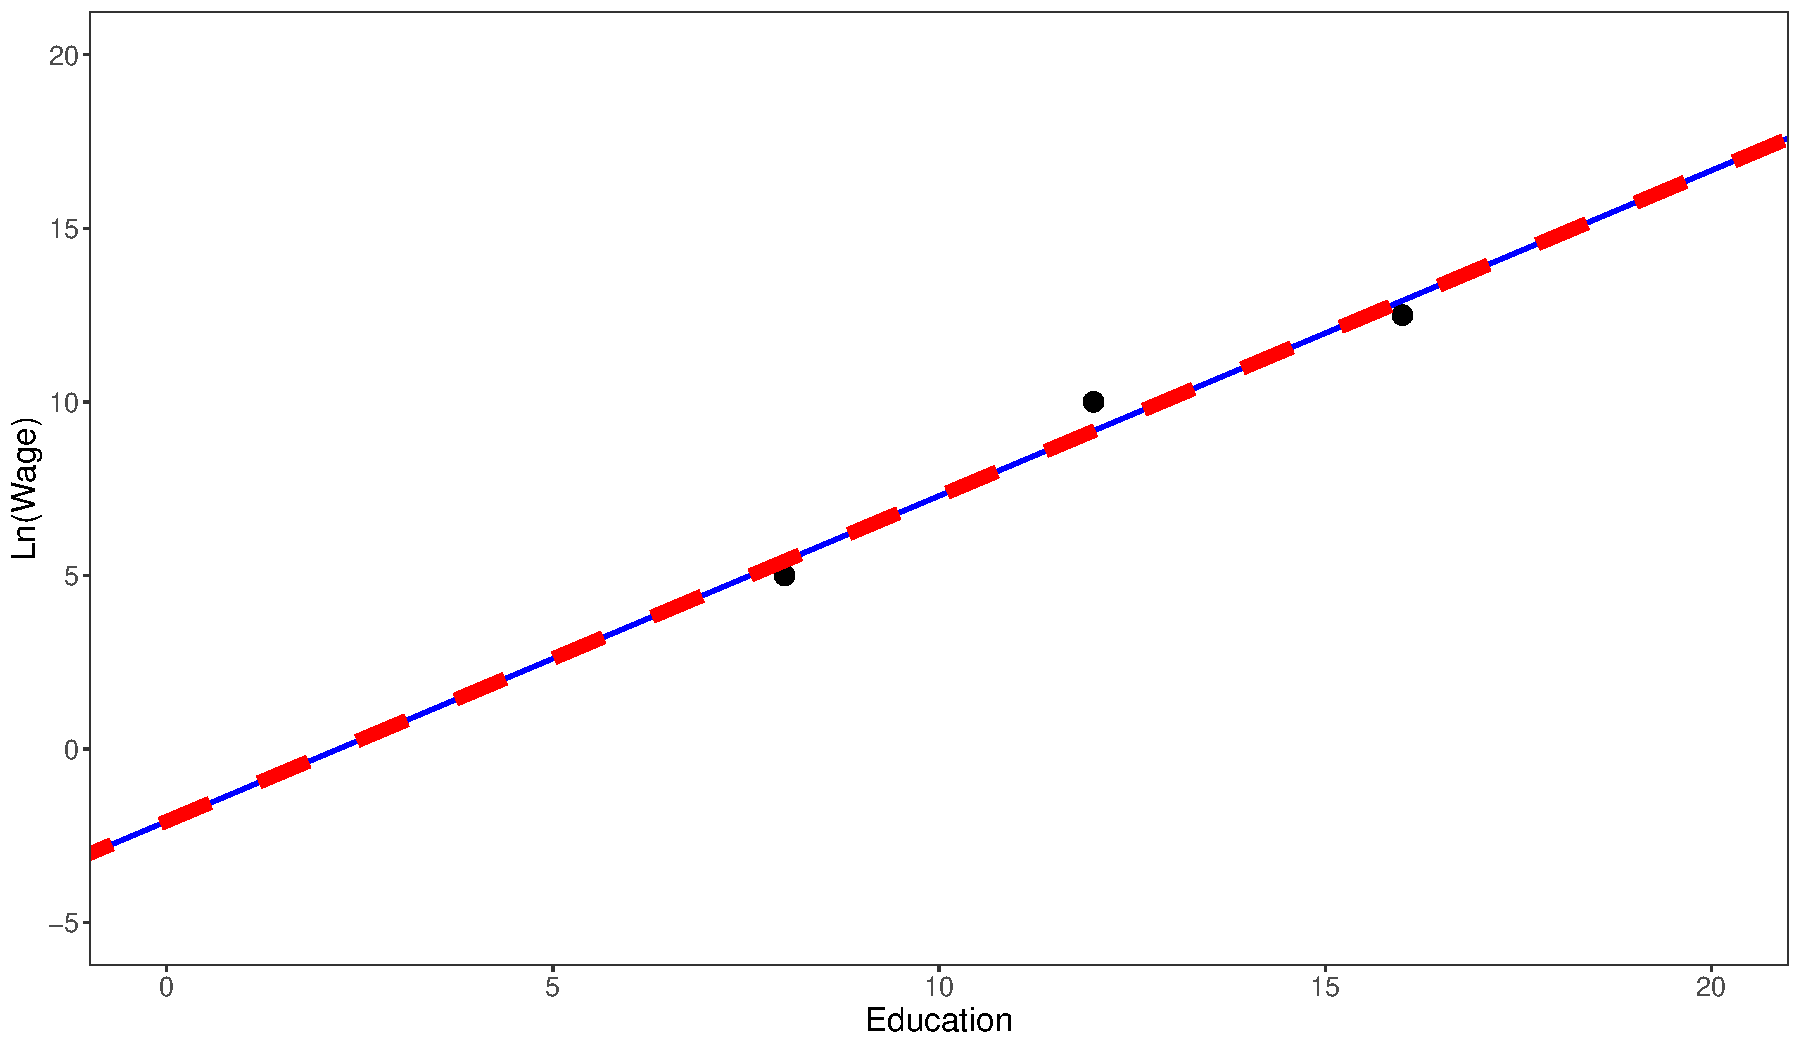
\includegraphics[scale=0.15]{figures/fig_1_7211.pdf}
    \end{figure}

 \end{frame}
 %----------------------------------------------------------------------%
\begin{frame}[fragile]
\frametitle{Stochastic Gradient-Based Optimization}

\begin{itemize}
  \item Computing the gradient can be very time consuming. 
  \item However, often it is possible to find a “cheap” approximation of the gradient. 
\begin{align}
  SSR=f(\theta)=\sum_{i=1}^{n}(y_{i}-(\alpha+\beta x_{i}))^{2} \nonumber \\
\theta_{j+1}=\theta_j -\epsilon_j \sum_{i=1}^n(\nabla_{\theta} f_i(\theta_j))\nonumber 
\end{align}


\item Approximating the gradient is still useful as long as it points in roughly the same direction as the true gradient.
\item We randomly typically without replacement) choose a subset of $\nabla_{\theta} f_i(\theta)$ for mini-batch gradient descent (mini-batch can be one)

\end{itemize}

 \end{frame}
 %----------------------------------------------------------------------%
\begin{frame}[fragile]
\frametitle{Stochastic Gradient-Based Optimization}
\begin{itemize}
 \item The key insight we only need taht $E(\nabla_{\theta} f_i(\theta_j))=\nabla_{\theta} f(\theta)$ 
\item  The word stochastic here refers to the fact that we acknowledge that we do not know the gradient precisely, but instead only know a noisy approximation to it. 



\begin{figure}[H] \centering
  \centering
  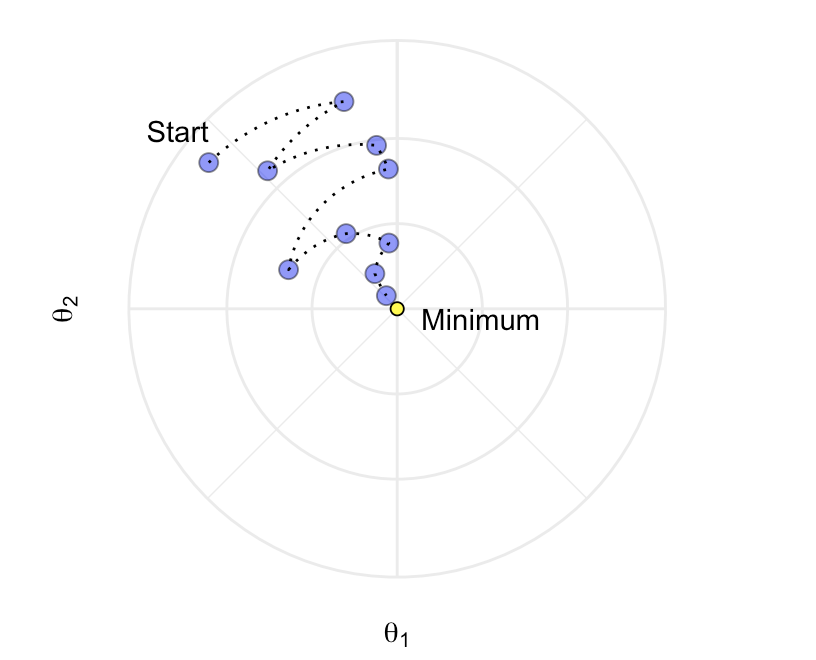
\includegraphics[scale=0.3]{figures/sgd.png}
  \\
  \tiny
  Source: Boehmke, B., \& Greenwell, B. (2019)
\end{figure}

\footnotesize
\item This makes the algorithm faster but 
\item Adds some random nature in descending the loss function’s gradient. 
\item Although this randomness does not allow the algorithm to find the absolute global minimum, it can actually help the algorithm jump out of local minima and off plateaus to get sufficiently near the global minimum.
\end{itemize}
\end{frame}
%----------------------------------------------------------------------%
\section{Parallel vs Distributed}
%----------------------------------------------------------------------%
\begin{frame}
\frametitle{Parallel vs Distributed}

\begin{itemize}
\item An algorithm is parallel if it does many computations at once. 
\begin{itemize}
  \item It needs to see all of the data
\end{itemize}
\medskip
\item It is distributed if you can work with subsets of data
\begin{itemize}
  \item \texttt{Stata-mp} is parallel. (license charges by core)
  \item \texttt{R} and \texttt{Python} can be parallel {\bf and} distributed
  \end{itemize}
\end{itemize}


\begin{figure}[H] \centering
  \centering
  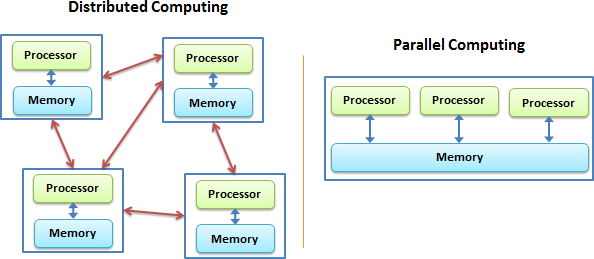
\includegraphics[scale=0.65]{figures/distributed_parallel.png}
  \\
  \tiny \url{https://tinyurl.com/y3nzvkwh}
\end{figure}


\end{frame}

%----------------------------------------------------------------------%
\begin{frame}
\frametitle{Map Reduce}

\begin{itemize}
  \item  Original Paper {\it MapReduce: Simplified data processing on large clusters (2004) Dean and Ghemawat}
  \medskip 
  \item It is of the most popular frameworks 
  \medskip
  \item Basic Idea:

  
\begin{enumerate}
  \item You need to be able to specify a key that indexes subgroups of data that can be analyzed in isolation.
  \item Map: Calculate and sort relevant statistics by key
  \item Partition and pipe the outcome of map so that outcomes with the same key end up on the same machine
  \item Reduce: Apply a summarization operation within the subgroup defined by each key.
\end{enumerate}
\end{itemize}



   
\end{frame}

%----------------------------------------------------------------------%
\begin{frame}
\frametitle{Example: Mean by groups}



\begin{figure}[H] \centering
  \centering
  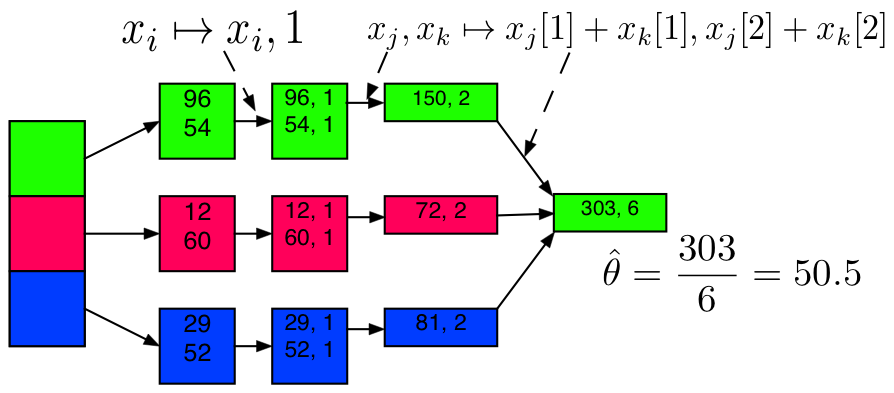
\includegraphics[scale=0.65]{figures/sketch_model_example.png}
  \\
  \tiny \url{https://datascienceguide.github.io/map-reduce}
\end{figure}

\end{frame}

%----------------------------------------------------------------------%
\begin{frame}[fragile]
\frametitle{\texttt{QR} decomposition for block matrices}
\tiny 
Idea on how to distribute OLS (Constantine \& Gleich, 2011)


\begin{align}
X_{8n\times k}=\left[\begin{array}{c}
X_{2n\times k}^{1}\\
X_{2n\times k}^{2}\\
X_{2n\times k}^{3}\\
X_{2n\times k}^{4}
\end{array}\right]
\end{align}


QR to each block

\begin{align}
X_{8n\times k}=\underset{8n\times4k}{\underbrace{\left[\begin{array}{cccc}
Q_{2n\times k}^{1}\\
 & Q_{2n\times k}^{2}\\
 &  & Q_{2n\times k}^{3}\\
 &  &  & Q_{2n\times k}^{4}
\end{array}\right]}}\underset{4k\times k}{\underbrace{\left[\begin{array}{c}
R_{k\times k}^{1}\\
R_{k\times k}^{2}\\
R_{k\times k}^{3}\\
R_{k\times k}^{4}
\end{array}\right]}}
\end{align}

\begin{align}
X_{8n\times k}=\underset{Q}{\underbrace{\underset{8n\times4k}{\underbrace{\left[\begin{array}{cccc}
Q_{2n\times k}^{1}\\
 & Q_{2n\times k}^{2}\\
 &  & Q_{2n\times k}^{3}\\
 &  &  & Q_{2n\times k}^{4}
\end{array}\right]}}\underset{4k\times k}{\underbrace{Q_{2}}}}}\underset{k\times k}{\underbrace{R_{2}}}
\end{align}

\end{frame}


%----------------------------------------------------------------------%
\begin{frame}
\frametitle{Spark}

\begin{itemize}
  \item  The tools facilitating distributed computing are rapidly improving. 
  \medskip
  \item One prominent system is Spark, that is quickly replacing MapReduce
  \medskip
  \item Seamlessly integration with \texttt{R} and \texttt{Python} and has it's own \texttt{MLlib}
  \medskip
  \begin{itemize}
   \item E.g. Spark uses distributed version of stochastic gradient descent to compute OLS  
   \medskip
    \end{itemize}       
    \item One of the key differences with MapReduce is how they load data 
    \medskip
    \begin{itemize}
     \item MapReduce has to read from and write to a disk
     \medskip
     \item Spark loads it  in-memory (can get 100x faster)
    \end{itemize}       

\end{itemize}    
  
\end{frame}

\begin{comment}
%----------------------------------------------------------------------%
\section{Motiviation Web Scraping}
%----------------------------------------------------------------------%
\begin{frame}
\frametitle{Motiviation Web Scraping}



\begin{figure}[H] \centering
  \centering
  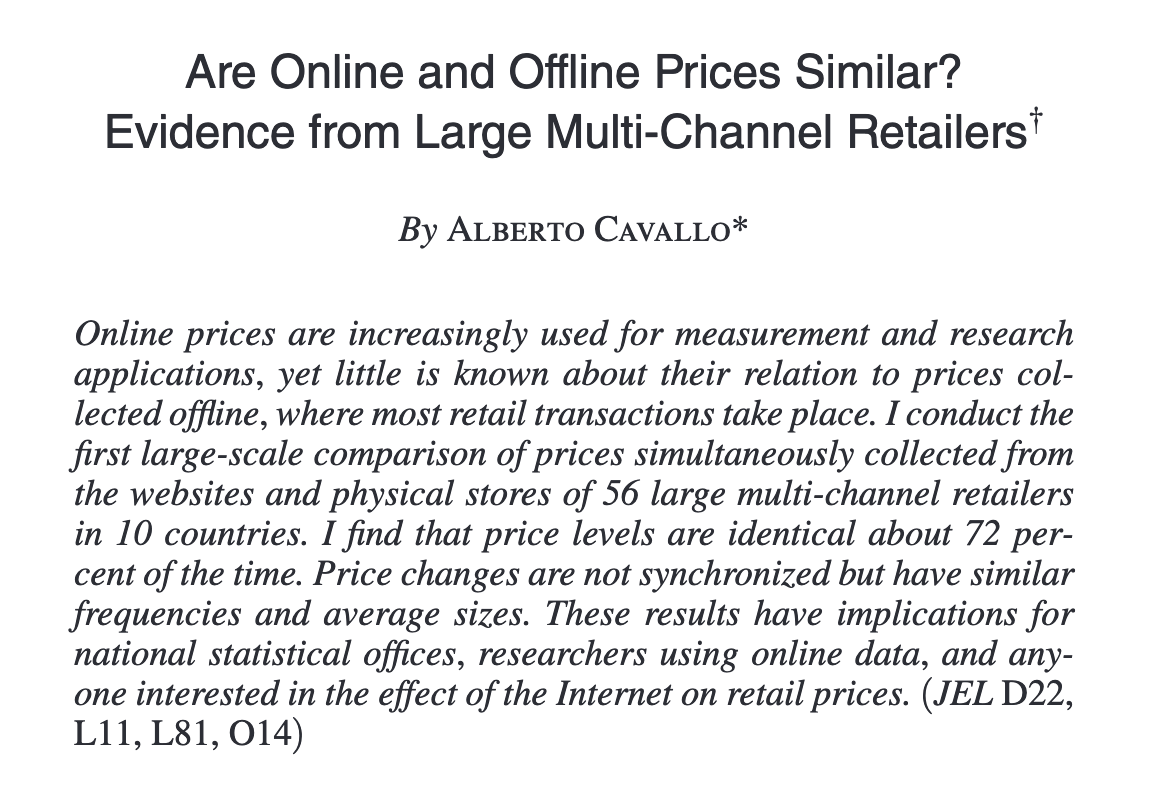
\includegraphics[scale=0.45]{figures/Cavallo_title}
  \\
  \tiny
\end{figure}
 

\end{frame}

%----------------------------------------------------------------------%
\begin{frame}
\frametitle{Motiviation Webscraping}



\begin{figure}[H] \centering
  \centering
  
\includegraphics[scale=0.25]{figures/Cunningham_title}
  \\
  \tiny
\end{figure}
 

\end{frame}

%----------------------------------------------------------------------%

\begin{frame}
\frametitle{Motiviation Webscraping}



\begin{figure}[H] \centering
  \centering
  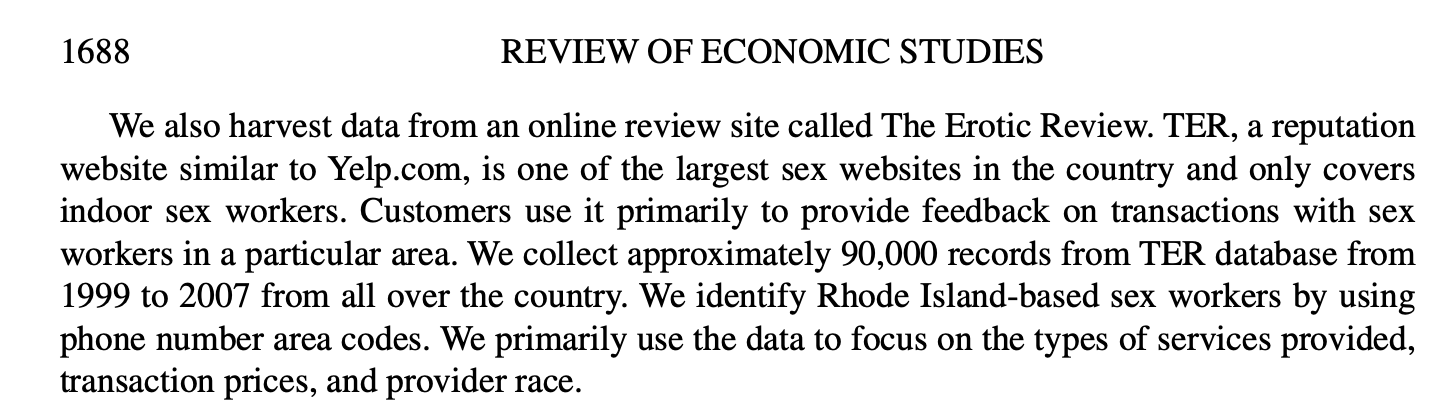
\includegraphics[scale=0.45]{figures/Cunningham_desc}
  \\
  \tiny
\end{figure}
 

\end{frame}


%----------------------------------------------------------------------%

\begin{frame}
\frametitle{Webscraping basics}

\begin{figure}[H] \centering
  \centering
  
\includegraphics[scale=0.75]{figures/webscrape_it.jpg}
  \\
  \tiny
\end{figure}

\end{frame}

%----------------------------------------------------------------------%
\begin{frame}
\frametitle{Webscraping basics}

\begin{itemize}
  \item How to get data, or "content", off the web and onto our computers.
  \bigskip
  \item If you see it in your browser it exists somewhere
  \bigskip
  \item To be ``successful'' one must have a working knowledge on:
  \begin{itemize}
  \item how web pages display content (Hyper Text Markup Language or HTML)
  \medskip
  \item where is the content ``located''


    \begin{enumerate}
    \item Server side
    \medskip
    \item Client side
    \medskip

    \end{enumerate}
    \item The good news is that both server-side and client-side websites allow for web scraping
   \end{itemize}
\end{itemize}





\end{frame}

%----------------------------------------------------------------------%
\begin{frame}
\frametitle{Caveat: ethical and legal limitations}

\begin{itemize}
\item Just because you *can* scrape it, doesn't mean you *should*. 
\medskip
\item Check \texttt{The Robots Exclusion Protocol} of a website, adding \texttt{``/robots.txt''} to the website's URL
\begin{enumerate}
  \item User-agent:  the type of robots to which the section applies
  \item Disallow:  directories/prefixes of the website not allowed to robots
  \item Allow:  sections of the website allowed to robots
\end{enumerate}
\medskip
\item \texttt{robots.txt} is de facto standard (see \url{http://www.robotstxt.org})
\medskip
\item Also always check the terms and conditions and what they say about scraping
\medskip
\item Remember the immortal words of uncle Ben: ``with great power comes great responsibility''

\end{itemize}


\end{frame}
\end{comment}
%----------------------------------------------------------------------%

\begin{frame}
\frametitle{Review \& Next Steps}
  
  \begin{itemize} 
    \item Computation
    \item QR decomposition
    \item Gradient Descent
    \item MapReduce and Spark
    %\item Intro to \texttt{Web Scraping}
    %\item Message: web scraping involves as much art as it does science
  \bigskip  

  
  \item  {\bf Next Class:} Problem Set Presentations
  \bigskip
  \item Questions? Questions about software? 
  
  \end{itemize}


\end{frame}


%----------------------------------------------------------------------%

\section{Further Readings}
%----------------------------------------------------------------------%
\begin{frame}
\frametitle{Further Readings}
\footnotesize
\begin{itemize}
  \item Boehmke, B., \& Greenwell, B. (2019). Hands-on machine learning with R. Chapman and Hall/CRC.
  \medskip
  \item Constantine, P. G., \& Gleich, D. F. (2011, June). Tall and skinny QR factorizations in MapReduce architectures. In Proceedings of the second international workshop on MapReduce and its applications (pp. 43-50).
  \medskip
  \item Dean, J., \& Ghemawat, S. (2004). MapReduce: Simplified data processing on large clusters.
  \medskip
  \item Deisenroth, M. P., Faisal, A. A., \& Ong, C. S. (2020). Mathematics for machine learning. Cambridge University Press.
  \medskip
  \item Goodfellow, I., Bengio, Y., Courville, A., \& Bengio, Y. (2016). Deep learning (Vol. 1, No. 2). Cambridge: MIT press.
  \medskip
  \item Van Loan, C. F., Golub, G. H. (2012). Matrix Computations. United States: Johns Hopkins University Press.
  \medskip
  \item \texttt{Webscraping} tutorial from  \href{https://grantmcdermott.com/}{Prof.~Grant McDermott}.
  \medskip
  \item \href{https://www.sas.upenn.edu/~jesusfv/Lecture_HPC_10_Web_Scrapping.pdf}{Web Scrapping slides} from Fernandez Villaverde J., Guerrón P. \& Zarruk Valencia, D. 
  
  
\end{itemize}

\end{frame}


\end{document}


